% -----------------------------------------------------------------------------
% !Mode:: "TeX:Hard:CP1252"
% PDFLaTeX this document and view or print it from Acrobat Reader!
% -----------------------------------------------------------------------------
% Preamble Starts here:
% -----------------------------------------------------------------------------
\documentclass[12pt,oneside,openany]{book}
\usepackage[cm]{fullpage}
\usepackage{blindtext}
\usepackage{graphicx}
\graphicspath{./SourceMaterial/} %Setting the graphicspath
%\usepackage[paperwidth=9.25in, paperheight=6.125in]{geometry}
\usepackage{makeidx}

\usepackage{amsmath}

\usepackage{hyperref}
\hypersetup{
%    bookmarks=true,         % show bookmarks bar?
    unicode=false,          % non-Latin characters in Acrobat�s bookmarks
    pdftoolbar=true,        % show Acrobat�s toolbar?
    pdfmenubar=true,        % show Acrobat�s menu?
    pdffitwindow=false,     % window fit to page when opened
    pdfstartview={FitH},    % fits the width of the page to the window
    pdftitle={My title},    % title
    pdfauthor={Author},     % author
    pdfsubject={Subject},   % subject of the document
    pdfcreator={Creator},   % creator of the document
    pdfproducer={Producer}, % producer of the document
    pdfkeywords={keyword1, key2, key3}, % list of keywords
    pdfnewwindow=true,      % links in new PDF window
    colorlinks=true,       % false: boxed links; true: colored links
    linkcolor=blue,          % color of internal links (change box color with linkbordercolor)
    citecolor=green,        % color of links to bibliography
    filecolor=cyan,         % color of file links
    urlcolor=magenta        % color of external links
}

%\usepackage{wrapfig}

%\usepackage{parskip}

\graphicspath{{Imagery/}} %Setting the graphicspath

%\includeonly{Poultry}

% Software names small caps
\newcommand{\windows}{\textsc{Microsoft Windows}}
\newcommand{\vstudio}{\textsc{Microsoft Visual Studio}}
\newcommand{\dbase}{\textsc{Microsoft Access}}
\newcommand{\excel}{\textsc{Microsoft Excel}}
\newcommand{\mut}{\textsc{Mut}}
\newcommand{\mf}{\textsc{Modflow}}
\newcommand{\mfu}{\textsc{Modflow-Usg}}
\newcommand{\mfus}{\textsc{Modflow-Usg$^{Swf}$}}
\newcommand{\tecplot}{\textsc{Tecplot}}
\newcommand{\github}{\textsc{GitHub}}
\newcommand{\ifort}{\textsc{Intel Fortran}}
\newcommand{\gb}{\textsc{Grid Builder}}
\newcommand{\gwv}{\textsc{Groundwater Vistas}}
\newcommand{\hgs}{\textsc{HydroGeoSphere}}

% Code, variable names san serif
\newcommand{\gwf}{\textsf{GWF}}
\newcommand{\cln}{\textsf{CLN}}
\newcommand{\swf}{\textsf{SWF}}

% Filenames, system commands typewriter texttt
\newcommand{\bin}{\texttt{USERBIN}}

\newcommand{\ins}[2]{
\includegraphics[width=0.3\textwidth]{BeginInstruction}
                     \squish
                     \begin{quote}
                        {\Large \sf #1 } \\
                        {#2  \rule{0.1in}{0.in}}
                     \end{quote}
                     \squish
                     
\includegraphics[width=0.3\textwidth]{EndInstruction}
                     \index{Input instructions ! #1}
                     }

\newcommand{\insp}[1]{\hspace*{.5in}{\sf #1} \\
                      \index{Input instructions ! #1} }


\newcommand{\squish} {\vspace*{-.2in}}

\newcommand{\str} [1] {\textbf{\$\_#1}}
\newcommand{\rnum} [1] {\textbf{R\_#1}}
\newcommand{\inum} [1] {\textbf{I\_#1}}



%\newcommand{\createspace}[2] {\vspace{.2in} \\ \includegraphics[width=#1\textwidth]{#2} \vspace{.2in} \\}

\makeindex

\begin{document}

% paragraph spacing
\setlength{\parindent}{.0in}
\setlength{\parskip}{.1in}
\setcounter{secnumdepth}{3}
\setcounter{tocdepth}{3}

\begin{titlepage}
    \vspace{1in}
    \centering
    \vfill
    {\bfseries\Huge
        Modflow User Tools (MUT) Version 1.31\\
         User's Guide\\
    }
    \vspace{.3in}

    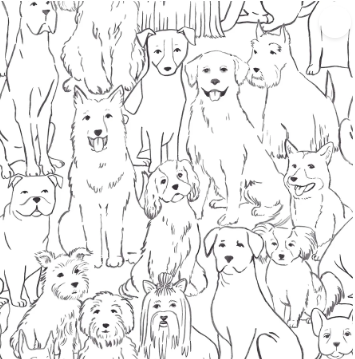
\includegraphics[width=0.8\textwidth]{mutts}

    \vspace{.3in}
    {\bfseries\Large
        October 2024\\
        \vskip2cm
        Rob McLaren, Young-jin Park, Sorab Panday\\
    }

    \vfill
    \vfill
\end{titlepage}

\pagestyle{empty} \tableofcontents

\pagestyle{plain}
\chapter{Introduction}\label{chapter:Introduction} This document describes a new \mfu\footnote{\url{https://www.gsienv.com/software/modflow-usg/modflow-usg/}}  development environment which has these features:
\begin{itemize}
    \item We refer to it as Modflow User Tools, or \mut\ for short.
    \item \mut\ is designed to work with a modified version of \mfu,  where a new surface water flow package, called \swf, has been added. Like the Connected Linear Network (\cln) package, the \swf\ package represents a new domain type that is fully-coupled to the 3D groundwater flow (\gwf) domain. There can also be cell-to-cell flows between the \swf\ and \cln\ domains.  The \swf\ domain uses the diffusion-wave approach so simulate 2D surface-water flow. We will refer to this new version of \mfu\ as \mfus\ in this manual.
    \item We currently develop and run it on a \windows\ 10-based computing platform, writing software using the \ifort\ compiler running inside the \vstudio\ interactive development environment, which includes software version control tools through \github.
    \item A text-based approach is used for the \mut\ interface, in which we first develop an input file of instructions that define our \mfus\ project,  then run \mut\ to read it and write a complete \mfus\ data set. \mut\ also writes output files for \tecplot, a third-party visualization software package, which provides a 3D graphical visualization tool to review the model numerical mesh and material properties in the data set. In future, \mut\ could be extended to support other third-party visualization packages, for example the open source program Paraview.
    \item \mut\ can post-process a \mfus\ simulation to provide a \tecplot\ visualization of temporal model results, including hydraulic heads, saturations, water depths and flow budget data.  \textit{If applied to output files which were produced by an earlier version of Modflow, results may be mixed.  It is not our intent here to support all existing Modflow packages, many of which have been superceded.}
\end{itemize}

This document is subivided into these sections:
\begin{description}
    \item[Chapter~\ref{chapter:Installation}]\textbf{Installation and Setup:} How to install \mut, \mfus\ and \tecplot\ and define \windows\ environment variables.
     \item[Chapter~\ref{chapter:ModelBuild}]\textbf{\mut\ Execution and Pre-processing} How to build a \mut\ input file, produce a \mfus\ compatible data set and \tecplot\ compatible output files with \mut, then review the results of the model build with \tecplot.
    \item[Chapter~\ref{chapter:ModelExecution}]\textbf{\mfus\ Execution and Post-Processing} How to run \mfus, convert the output to \tecplot-compatible files with \mut, then visualize them with \tecplot.
    \item[Chapter~\ref{chapter:ModelVerification}]\textbf{Model Verification} Examples used to verify the accuracy of \mfus\ models built using \mut.
    \item[Chapter~\ref{chapter:IllustrativeExample}]\textbf{Illustrative Example} An example which illustrates the use of \mut\ and \mfus\ to simulate variably-saturated, fully-coupled   \gwf\-\swf\ flow in a large-scale watershed.
    \item[Appendix~\ref{Appendix:ExcelUseage}]\textbf{\excel\ Database Files} Details about using the provided \excel\ database files, which are currently used to store \mfus\ model material property and solver parameter data sets.
    \item[Appendix~\ref{Appendix:TecplotUseage}]\textbf{\tecplot\ Useage} Details about using \tecplot\ to visualize output files generated by \mut\ during model build and execution.
        \end{description} 

\chapter{Software Installation and Useage}\index{Installation}
\begin{enumerate}
    \item Obtain the MUT source files from:
        \begin{verbatim}
            https://github.com/Grdbldr/MUT_Source.git
            https://github.com/Grdbldr/MUT_Examples.git
        \end{verbatim}

    \item Define a windows environment variable USERBIN e\.g\.:
        \begin{verbatim}
            set USERBIN=c:\program_files\bin
        \end{verbatim}
        This can be done through Windows settings or at the command prompt.

    \item Build the source in Microsoft Visual Studio.  We provide a Visual Studio 2019 solution file for this purpose. Currently, Microsoft is providing a free community version of Visual Studio 2022 but we haven't yet tested this version.  Please let us know how this works if you try it.

\end{enumerate}   

\chapter{Model Build}\label{chapter:ModelBuild}
The first step in any model build is to develop a conceptual model, which defines the extent, inflows and outflows, material distributions and physical properties of a hydrogeologic flow system, real or imaginary. The intent of \mut\ is to then facilitate the production of a set of \mfus\ input files by minimizing the amount of time we spend building and testing it.  This chapter describes our current model build workflow, which can provide a sound basis for developing your own personal workflow.

The steps in our model build workflow are:
\begin{enumerate}
    \item Create a new working folder or copy an existing \mut\ project folder. \label{step:copy}
    \item Modify the \mut\ input file (and other input files if necessary) to reflect the new Modflow project.\label{step:modify}
    \item Run \mut\ to build the new Modflow project, which also produces \tecplot\ output files for the various Modflow domains (i.e. \gwf, \swf\ and/or \cln ) created during the build process. \label{step:mut1}
    \item Run \tecplot\ and examine the build output files.   \label{step:Tecplot1}
    \item Repeat steps~\ref{step:modify}-\ref{step:Tecplot1} until the new project is defined to your satisfaction.
\end{enumerate}

A \mut\ input file is a plain ascii text file that you can edit with your preferred editor (e.g. Windows Notepad\footnote{Our personal favourite editor is WinEdt (\url{https://www.winedt.com/snap.html}), which also provides a nice \LaTeX\ document development environment when coupled with the \TeX\ software package MiKTeX.  This manual was produced using these word processing tools.}).
The \mut\ input file name can have a prefix of your choice, followed by the extension \texttt{.mut}. Examples of valid \mut\ input file names are \texttt{\_build.mut} or \texttt{good.mut}. Most often, the easiest approach is to copy an existing input file and modify it as required.  This helps reduce set-up time and avoid potential errors that are introduced when creating input files from scratch.

To illustrate our model build workflow, we will refer to the various conceptual models developed for our existing suite of examples described in  Chapter~\ref{chapter:ModelVerification}.  As you read along, we urge you to carry out the steps we describe as we move through the workflow.  We recommend copying the contents of an existing model to a new location (e.g.\ copy the folder \texttt{1\_VSF\_Column} to \texttt{C:$\backslash$SandBox}).
\pagebreak 
If you did so, your working directory would look something like this:

    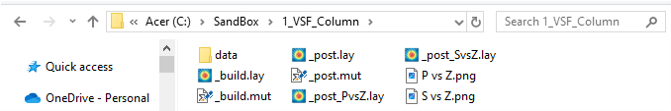
\includegraphics[width=\textwidth]{3_1_vsf_column_folderinit}

In the \texttt{1\_VSF\_Column} example, there is a \mut\ input file for the model build called \texttt{\_build.mut} and a \tecplot\ layout file called \texttt{\_build.lay} used to visualize the model build results.  The rest of the files are related to post-processing \mfus\ model results and will be discussed later in chapter~\ref{chapter:ModelExecution}.
 
 In our preferred workflow we would first start a command prompt in the folder which contains the \mut\ input file by:
\begin{enumerate}
   \item  Navigating to the folder in File Explorer (e.g.\ \texttt{C:$\backslash$SandBox$\backslash$1\_VSF\_Column}).
   \item  Highlighting the path in File Explorer:

        
\includegraphics[width=0.3\textwidth]{3_3_HighlightPath}

    \item  Replacing the existing path with the string {\sf cmd}:

        
\includegraphics[width=0.5\textwidth]{3_4_cmd}

    \item Pressing Enter/Return.
\end{enumerate}
A command prompt window rooted at the input folder should appear:

        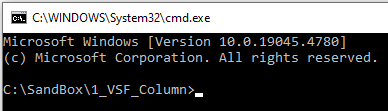
\includegraphics[width=0.4\textwidth]{3_5_cmdPrompt}



When you run \mut\, it will try to obtain a prefix in the following order:
\begin{enumerate}
    \item \textbf{From a command line argument:} \label{commarg} At the command prompt, \mut\ checks for the presence of a command line argument.  For example, typing this:
\begin{verbatim}
    mut Good
\end{verbatim}
        would cause \mut\ to process the input file \texttt{Good.mut}.
    \item \textbf{From a prefix file:} If there is no command line argument, \mut\ checks for the presence of the file \texttt{\_mut.pfx} in the folder.  If present, \mut\ will read the prefix from it. For example, if the mut file was called \texttt{Good.mut} then the file \texttt{mut.pfx} would contain the single line:
\begin{verbatim}
    good
\end{verbatim}
    \item \textbf{From the default input file:} If there is no command line argument or prefix file in the folder, \mut\ checks for the presence of the file \texttt{a.mut}.  If present in the folder, \mut\ will process it.
    \item \textbf{From the keyboard:} If none of these methods are successful, \mut\ will prompt for a prefix as shown here:

        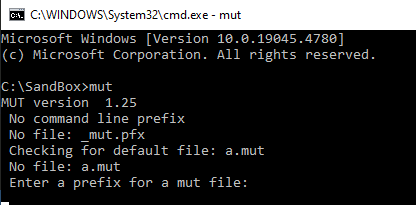
\includegraphics[width=0.6\textwidth]{3_2_mut_no_prefix}

        The user would type the prefix e.g.: \texttt{good} and press Enter.

\end{enumerate}

To build the \texttt{1\_VSF\_Column} example, we would  run \mut\ using the input file \texttt{\_build.mut} by typing:
\begin{verbatim}
    mut _build
\end{verbatim}
which uses the first method to supply the prefix.


If you open the file \texttt{\_build.mut} in a text editor you will see the first couple of lines are comments (which begin with an exclamation point character: '{\tt !}') describing the problem:
\squish
\begin{verbatim}
    ! Examples\1_VSF_Column:
    !   A modflow project of a 1D column generated from a simple 2d rectangular mesh
\end{verbatim}
 \mut\ first creates a clean copy of the input file called \texttt{\_buildo.input} by removing all comment lines.

 As \mut\ processes the input file, output is written to both the screen and to the file \texttt{\_buildo.eco}.  If you open \texttt{\_buildo.eco}, you will see the first thing written is the \mut\ header, which contains the version number and build date.

 These are followed by the stripped comments, which  can provide a synopsis of the input file contents. The rest of the cleaned input file contains \mut\ instructions, which may require data in the form of numbers (e.g.\ parameter values) or alphanumeric strings (e.g.\ file names).


The first instruction in the cleaned input file begins the model build:

\ins{build modflow usg}
    {This  is a {\em subtask} that defines the characteristics of the \mfus\ model including:
     \begin{itemize}
        \item Units of length and time.
        \item Numerical model meshes.
        \item Material properties.
        \item Boundary conditions.
        \item Time-stepping, stress period and output control parameters.
        \item Solver parameters.
    \end{itemize}

    An end instruction is required to stop the subtask e.g.:

    {\Large \sf end build modflow usg}
    }

After \mut\ finishes, the working folder should look something like this:

        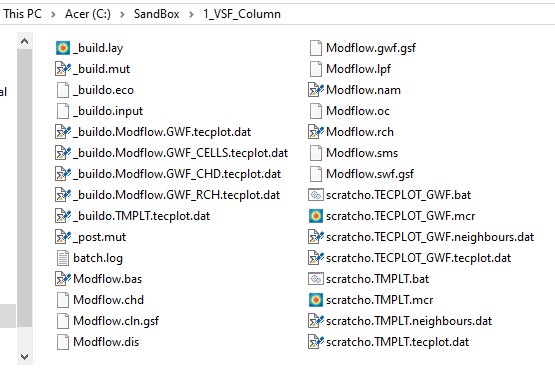
\includegraphics[width=0.8\textwidth]{3_6_buildFiles}

Several new output files have been created, of which it may be noted:
\begin{itemize}
    \item Build output files, which have the prefix \texttt{\_buildo}, appear near the start of the list if sorted by name. \mut\ deletes previously generated build output files and writes a fresh set each time it is run.  This can prevent confusion that might arise if out-of-date output files were present.\footnote{For example, if we define a recharge boundary condition, \mut\ will create the file \texttt{\textit{prefix}o.Modflow.SWF\_RCH.Tecplot.dat} which shows the locations and recharge values assigned to Modflow cells.  If we then removed the recharge condition from the input file, but did not delete this output file, we may assume the recharge condition still applies.}
    \item \tecplot\ output files are indicated by the suffix \texttt{.tecplot.dat}.
    \item Modflow model input files are written using the default prefix \texttt{Modflow}, (e.g.\ \texttt{Modflow.nam, Modflow.bas} etc.)  The prefix can be customized if desired but there are advantages to keeping this 'generic' one, such as portability of post-processing scripts or \tecplot\ layout files that follow this generic naming convention.
    \item Several scratch files (with prefix \texttt{scratcho}) are written. These are used for debugging during code development and can be ignored in most cases.
    \item If the run is successful the last line written will be \texttt{Normal exit}, otherwise an error message will be given.
\end{itemize}


    \section{Defining the Units of Length and Time}\label{section:Units}
The input files written by \mut\ define the units of length and time that are applied during the \mfus\ model simulation.

By default, \mut\ assigns meters as the units of length and seconds as the units of time. If desired, the following instructions can be used to define a different unit system:

\ins{units of length}
    {
        \squish
        \begin{enumerate}
        \item \str{LengthUnits}  The desired units of length.
        \end{enumerate}
        \mfus\ currently supports length units of feet, meters or centimeters.
        }

\ins{units of time}
    {
        \squish
        \begin{enumerate}
        \item \str{TimeUnits}  The desired units of time.
        \end{enumerate}
        \mfus\ currently supports time units of seconds, minutes, hours, days or years.
    }

These instructions would define units of centimeters and days instead of meters and seconds:
 \begin{verbatim}
    units of length
    centimeters

    units of time
    days
 \end{verbatim}

\mut\ converts the string variables \str{LengthUnits} and \str{StringUnits} to their numeric equivalents and passes that to \mfus\ through the variables \textsf{LENUNI} and \textsf{ITMUNI} respectively.

    \section{Defining the Template Mesh}\label{texfile:TemplateMesh}
The next step in the model build workflow is to define a template mesh, which is a 2D finite-element mesh that is used to generate a 3D \gwf\ (and possibly a 2D \swf) finite-element mesh.   Below is an example
\footnote{This example was generated using the \tecplot\ layout file \texttt{MUT\_Examples$\backslash$6\_Abdul\_Prism\_Cell$\backslash$FIG Template Abdul.lay}. }
  showing an exploded view of a template mesh (bottom image) that was used as a basis for generating  finite-element meshs for the \gwf\ (middle image) and\swf\ (upper image) domains:

    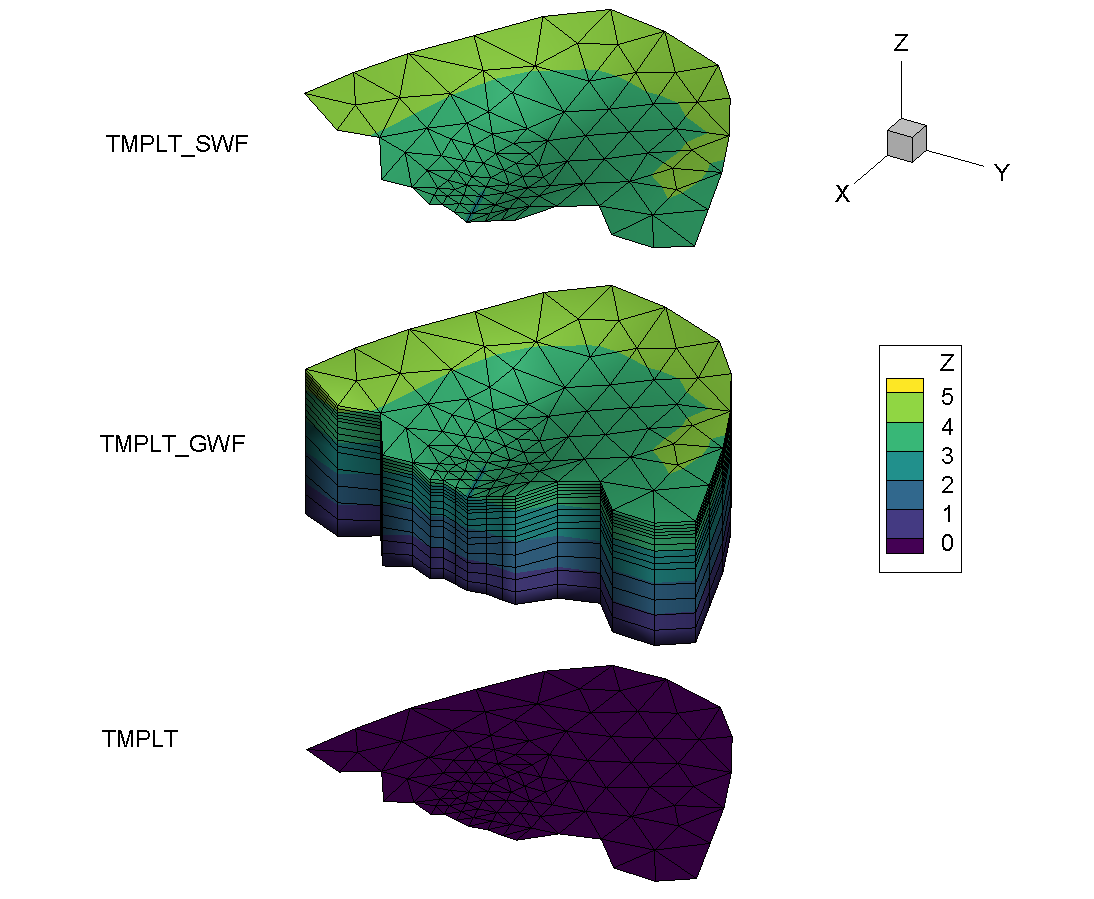
\includegraphics[width=0.87\textwidth]{3_7_tmpltAbdul}

Some key features of this example are:
\begin{itemize}
  \item The template mesh is assigned an elevation of zero, and only the $xy$ coordinate data are used to define the other domains.
  \item The \gwf\ domain has been assigned a base elevation of zero, and a variable top elevation.
  \item The \swf\ domain has been assigned the same elevation as the \gwf\ domain i.e.\ they are coincident.
\end{itemize}

\pagebreak
 In this example, the template mesh was defined using these instructions:
 \squish
\begin{verbatim}
    2d mesh from gb
    .\gb\grid
\end{verbatim}
The instruction \textsf{2d mesh from gb}, which requires a single line of input, \texttt{.$\backslash$gb$\backslash$grid}, is documented as shown here:

\ins{2d mesh from gb}
    {
        \squish
        \begin{enumerate}
        \item \str{Prefix}  The \gb\ \footnote{\gb\ is a legacy 2D triangular finite-element grid generator.} dataset prefix, including the path to it.
        \end{enumerate}
        Given \str{Prefix}, this instruction reads the 2D finite-element grid data and uses it to define the 2D template mesh.  \str{Prefix} should contain a relative path to the dataset.  Examples of relative paths are:
        \begin{description}
        \item[.$\backslash$gb$\backslash$grid] The \mut\ input folder contains a local folder \texttt{gb} with the data set prefix \texttt{grid}.
        \item[..$\backslash$gb$\backslash$grid] The parent folder to the \mut\ input folder contains a folder \texttt{gb} with the data set prefix \texttt{grid}.
        \item[C:$\backslash$gb$\backslash$grid] Absolute path to a drive \texttt{C:} with a folder \texttt{gb} with the data set prefix \texttt{grid}.  Absolute paths are not recommended as they may lead to portability issues.
        \end{description}
        \squish
    }

To generate uniform 2D rectangular element template meshes \footnote{See for example the verification cases \texttt{MUT\_Examples$\backslash$1\_VSF\_Column} or \texttt{MUT\_Examples$\backslash$6\_Abdul\_MODHMS}} use this instruction:

\ins{generate uniform rectangles}
    {\index{generate uniform rectangles}
    \squish
    \begin{enumerate}
    \item \rnum{xl}, \inum{nbx}  Domain length and number of blocks in the $x$-direction
    \item \rnum{yl}, \inum{nby}  Domain length and number of blocks in the $y$-direction
    \end{enumerate}
    A 2D finite-element mesh composed of uniform rectangular elements will be generated. In this case, the
    grid is formed by subdividing the domain in the $x$-direction into \inum{nbx} blocks, each of length
    \textbf{\rnum{xl}/\inum{nbx}}. The domain is subdivided in a similar fashion in the $y$-direction, using the other input parameters.
    }

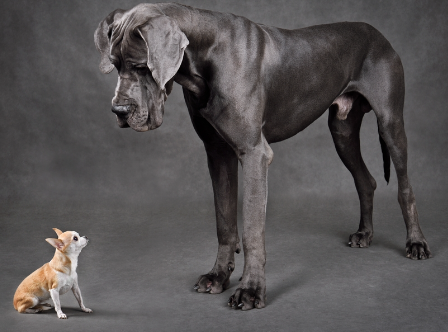
\includegraphics[width=.15\textwidth]{ModelDevelopment} \textit{Do we have a working quadtree example to add here as an option.}
%This instruction reads a quadtree mesh to define a template mesh \footnote{See for example the verification case \texttt{UNDER CONSTRUCTION}}:
%
%\ins{2d quadtree mesh from groundwater vistas}
%    {\index{2d quadtree mesh from groundwater vistas}
%    \squish
%    \begin{enumerate}
%    \item \textbf{gbprefix}  The \gwv\ \footnote{\gwv\ is  third-party \mf\ development environment software.} dataset prefix, including the path to it.
%    \end{enumerate}
%    Given \textbf{gbprefix}, this instruction reads the 2D finite-element grid data and uses it to define the 2D template mesh.  The prefix should contain a relative path to the dataset.  Examples of relative paths to a Grid Builder prefix variables are:
%
%    
\includegraphics[width=.15\textwidth]{UnderConstruction}
%    }

There are two ways that \mf\ cell control volumes can be defined from the template mesh.  By default, \mut\ uses a mesh-centred approach as shown here for a triangular-element template mesh:

    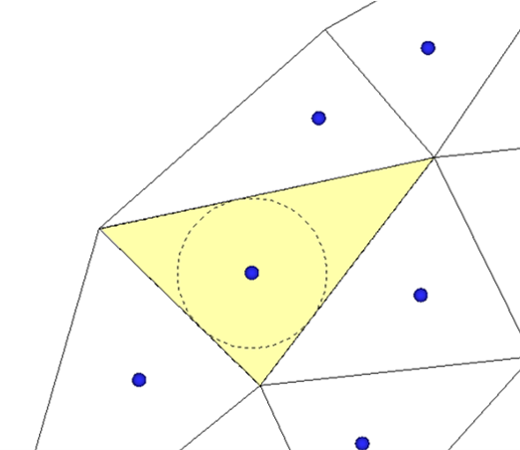
\includegraphics[width=0.6\textwidth]{3_8_MeshCentred}

Some key features to note are:
    \label{page:MeshCentredApproach}
    \phantomsection\label{page:MeshCentredApproach}.
\begin{itemize}
    \item Inner circles, which are tangent to all three element sides, are defined for each triangular element.  An example is shown by the dashed circular line in the yellow-shaded element.
    \item The blue-filled circles show the locations of the defined \mf\ cell control volumes.
    \item The vertical connection area of the cell is defined by the triangular element area (yellow-shaded triangle).
    \item The horizontal connection length of the cell is defined by the triangular element side length between neighbouring elements.
\end{itemize}

The mesh-centred approach is similar when using a  rectangular-element template mesh, with the rectangular element area and side lengths defining the vertical connection area and horizontal connection length respectively.

\pagebreak
To use a node-centred control volume approach, add this instruction {\em before} defining any \gwf\ or \swf\ model domains:

\ins{nodal control volumes}
    {The node-centered approach will be used to define \mf\ cell centres instead of the default mesh-centered approach.
     }

The result of using a node-centred approach is shown here for a triangular-element template mesh:

    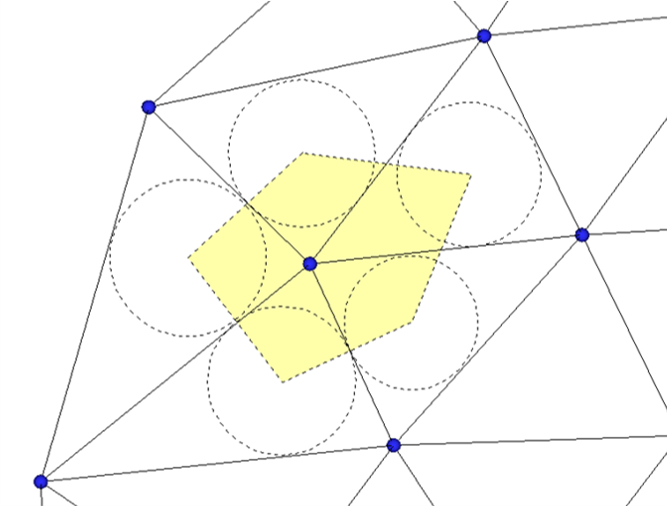
\includegraphics[width=0.6\textwidth]{3_9_NodeCentred}

Some key features to note are:
    \label{page:NodeCentredApproach}
    \phantomsection\label{page:NodeCentredApproach}.
\begin{itemize}
    \item The blue-filled circles show that the locations of the defined \mf\ cell control volumes are now located at template mesh node locations.
    \item The vertical connection area of the cell (yellow-shaded polygon) is defined by the contributing area formed by joining the inner circle centres of each element containing the template mesh node.         \label{page:NodeCentredApproach}
    \item The horizontal connection length of the cell is defined by the distance to a neghbouring node.
\end{itemize}


\includegraphics[width=.15\textwidth]{UnderConstruction} \textit{Should explain how inner circle radius is used for connection length and perpendicular area for triangles.}




    \section{Groundwater Flow(\gwf) Domain}\label{texfile:GWF}
Currently, every \mfus\ model must contain a \gwf\ domain, which may be reduced to a single layer of very low hydraulic conductivity in cases where \gwf\ flow and interaction with other model domains is to be neglected.

\subsection{Generating a Layered \gwf\ Domain}
A \mfus\ 3D groundwater flow (\gwf) domain can be generated from the template using this instruction:

\ins{generate layered gwf domain}
    {This subtask has instructions that are used to define:
     \begin{itemize}
        \item Element zone numbering scheme
        \item Top elevation (i.e. $z$-coordinate)
        \item Mesh layers and vertical discretization
    \end{itemize}

    Subtask instructions will be read and processed until an \textsf{end} instruction is encountered.  We suggest appending the subtask name to the \textsf{end} instruction:

    {\Large \sf end generate layered gwf domain}
    }

The construction of the 3D \gwf\ finite-element mesh proceeds from top to bottom.  First, we define the top elevation, then add layers one at a time until we reach the base of the domain. By default, element zone numbers will be assigned by layer number.  If the template mesh is divided into horizontal patches with unique zone numbers, these can be assigned instead to the 3D GWF mesh \footnote{The verification example \texttt{MUT\_Examples$\backslash$6\_Abdul\_Prism\_Cell} uses this option to define \swf\ domain zones.} using this instruction:

\ins{Zone by template}
    {Causes \mut\ to assign the template mesh element zone number to the corresponding 3D \gwf\ element.

    {\em This instruction should appear in the input file at the beginning of the \textsf{generate layered gwf domain} subtask before new layers are added.}
    }

\subsubsection{Defining the Top Elevation} \label{section:topelev}
To assign an elevation to the top layer of template nodes use this instruction:

\ins{top elevation}
    {This subtask defines the elevation (i.e. $z$-coordinate) of the top layer of nodes in the \gwf\ finite-element template mesh in one of these ways:
     \begin{itemize}
        \item By assigning a given elevation to all nodes
        \item By reading variable elevation data from a file
        \item By interpolating elevation data from a function $z(x)$ where the elevation $z$ varies by the nodes $x$ coordinate.
     \end{itemize}
     Once the elevation is defined, an \textsf{end} instruction is required to stop the subtask e.g.\:

    {\Large \sf end top elevation}
    }

 The top elevation can be defined by one of these instructions: \label{'Page:TopElev'}

 \ins{elevation constant}
    {\squish
    \begin{enumerate}
    \item \rnum{elev}\  The elevation \rnum{elev}\ will be assigned to all top layer nodes.
    \end{enumerate}
    \squish
    }

 \ins{elevation from gb file}
    {\squish
    \begin{enumerate}
    \item \str{file}\  The elevation data in the \gb\ nodal property file named \str{file}\ will be assigned to the top layer nodes.
    \end{enumerate}
    \squish
    }

The \gb\ nodal property file uses a legacy binary file format. You can develop your own ascii input files and read them using this instruction:

 \ins{elevation from list file}
    {\squish
    \begin{enumerate}
    \item \str{file}\  The elevation data in the ascii file named  \str{file}\ will be assigned to the top layer nodes.
    \end{enumerate}
    \squish
    }

Part of a sample list file \footnote{The verification example \texttt{MUT\_Examples$\backslash$6\_Abdul\_MODHMS} uses an ascii file input to define nodal elevations.} is shown here:
    \begin{verbatim}
    Kriged cell top elevation for layer 1
     4.414571762E+000
     4.415914536E+000
     ...
     4.415914536E+000
     \end{verbatim}
     \squish
Some key features of this example are:
\begin{itemize}
  \item The first line of the file is discarded, and in this case contains a string describing the data.
  \item You must supply a value for each node in the template finite-element mesh.
  \item The data is read in free format so there can be more than one value entered per line.
  \item Only the start and end of the file are shown here, with the string '\texttt{...}' replacing the middle portion.
\end{itemize}

To define the top elevation as a function of $x$ (usually used for cross-sectional models) use this instruction:

 \ins{elevation from xz pairs}
    {
    \squish
    \begin{enumerate}
    \item \rnum{x(1)}, \rnum{y(1)}  First $x, z$ coordinate pair.
    \item \textbf{...}
    \item \rnum{x(n)}, \rnum{y(n)}  nth $x, z$ coordinate pair.
    \end{enumerate}

     An elevation is calculated for each chosen cell, based on it's $x$-coordinate location, by interpolating an elevation from the given list of  $xz$-coordinate pairs.

     This subtask reads a list of $xz$-coordinate pairs until an \textsf{end} instruction is encountered e.g.\:

    {\Large \sf end elevation from xz pairs}
    }

Here is an example showing the use of this instruction \footnote{The verification example \texttt{MUT\_Examples$\backslash$1\_VSF\_Hillslope} uses the \textsf{elevation from xz pairs} pairs instruction to define the top elevation of the cross-sectional domain.}:
    \begin{verbatim}
    elevation from xz pairs
           0.0, 0.0
        1000.0, 100.0
    end elevation from xz pairs
     \end{verbatim}
     \squish
Some key features of this example are:
\begin{itemize}
  \item The two given $xz$ pairs define a line that slopes from $z=0$ at $x=0$ to $z=100.0$ at $x=1000$.  You may supply as many pairs as needed to define the top of your cross-section.
  \item $x$ coordinates must increase continuously from the top of the list to the bottom.
  \item the $x$-range of the supplied pairs should cover the entire $x$-range of the template mesh.
  \item For each node in the template mesh, the $x$ coordinate is used to interpolate an elevation (i.e. $z$ value) using the appropriate $xz$ pair.
\end{itemize}

\subsubsection{Adding Layers} \index{\gwf\ Domain ! layering}
    {\em NOTE: The term layers used here should not be confused with the \mf\ term of the same name. A \mf\ layer is one cell thick, while a \mut\ layer can be one or more elements thick.}

A \mfus\ model must contain at least 1 layer, and each layer is defined using this instruction:     {\index{Grid generation ! \gwf\ Domain ! New layer}

\ins{new layer}
    {This subtask adds a new layer to the \gwf\ domain by defining the layer:
     \begin{itemize}
       \item Base elevation
       \item Vertical discretization
     \end{itemize}

     It reads instructions until an \textsf{end} instruction is found e.g.\:

    {\Large \sf end new layer}
    }

The base elevation is defined using the elevation instructions  described on page~\pageref{'Page:TopElev'} that are given for the \textsf{top elevation} instruction.

By default, a new layer will be assigned the name '\texttt{Layer {\em n}}' where {\em n} is the current layer number.  If you want to assign your own layer name use this instruction:

\ins{Layer name}
    {
    \squish
    \begin{enumerate}
    \item \str{layer\_name} Layer name.
    \end{enumerate}
    \squish
    }

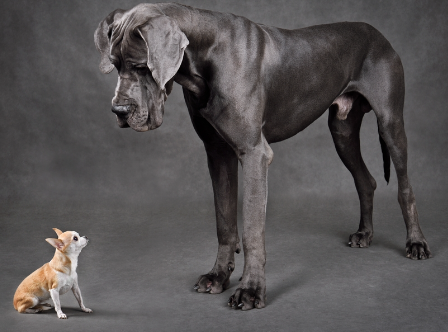
\includegraphics[width=.15\textwidth]{ModelDevelopment} \textit{These names are not currently used in Tecplot output but could/should? be used to create the customlables for zone naming.}



By default, \mut\ will stop and issue a warning message if the computed layer base elevation is greater than or equal to the current layer top elevation.  This instruction forces the base to be below the top by a set amount:

\ins{Minimum layer thickness}
    {\squish
    \begin{enumerate}
    \item \rnum{MinThick} Minumum thickness value[L].
    \end{enumerate}
    This instruction causes \mut\ to enforce a minimum thickness constraint for the current layer. At nodes where the computed layer base elevation is greater than or equal to the current top elevation, \rnum{MinThick} will
    be subtracted from the current top elevation to get the base elevation.
    }

By default, a new layer will not be subdivided vertically unless one the following two instructions is issued.
The first creates a uniform subdivision:

\ins{Uniform sublayering}
    {\squish
    \begin{enumerate}
    \item \inum{nsublayer} Number of sublayers.
    \end{enumerate}
    This instruction divides the layer vertically into \inum{nsublayer}
    elements, which will each have the same element height, equal to the top elevation
    minus the current base elevation divided by \inum{nsublayer}.
    }

This instruction creates a non-uniform subdivision:

\ins{Proportional sublayering}
    {\squish
    \begin{enumerate}
        \item \inum{nsublayer}  Number of proportional sublayers.
        \item \rnum{sub\_thick(i),i=1,\inum{nsublayer}} Proportional thicknesses in order from top to bottom.
    \end{enumerate}
    This instruction can be used if you want to refine the \gwf\ domain mesh vertically,
    for example, in the active zone with the \swf\ domain the ground surface in the .

    It is important to understand that the variable \rnum{sub\_thick} is not
    a true thickness, but is instead a relative thickness, which is used along
    with the layer thickness to determine the element heights in the current
    column.

}

    For example, these instructions:
    \texttt{
            \begin{tabbing}
            AAA\=AAA\=AAA   \kill
                \>Proportional sublayering   \\
                \>   \> 3                     \\
                \>   \> 0.1           \\
                \>   \>1.0            \\
                \>   \>  10.0       \\
                \> end       \\
            \end{tabbing}
    }
    \squish
would subdivide the current layer vertically into three elements, between
    the current base and top elevation, with element height proportions of .1,
    1 and 10 from top to bottom.

This instruction is most often used to define a layer of uniform thickness relative to an uneven top elevation:

\ins{Offset base}
    {\squish
    \begin{enumerate}
    \item \rnum{value} Thickness value (L) by which to offset the layer base elevation.
    \end{enumerate}
    This instruction causes the elevation of the base of the layer to be offset vertically by the given value.  This
    can be used to create a surface a given distance below another surface.
}

    For example, these instructions:
\begin{verbatim}
        top elevation
            elevation from list file
            elev.list
        end top elevation

        new layer
            uniform sublayering
            3

            elevation from list file
            elev.list

            offset base
            -1.0

        end new layer

    end generate layered gwf domain
\end{verbatim}
 create a layer with a top elevation 1 metre below the elevation defined in the raster file \texttt{elev.list}:


\includegraphics[width=.15\textwidth]{UnderConstruction} \textit{Need to check sign on \textsf{offset base} input}

\subsubsection{Cell Connection Properties}  \index{\gwf\ Domain ! cell connection properties}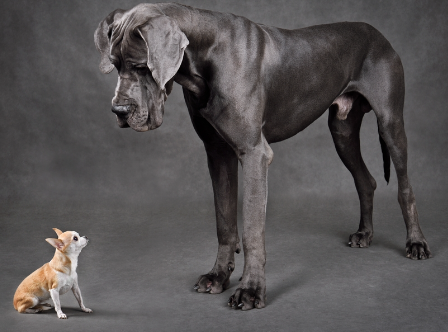
\includegraphics[width=.15\textwidth]{ModelDevelopment} \textit{
\gwf\ cell to \gwf\ cell connection properties are automatically defined by \mut\ based on control-volume approach and element type. The code needs to be checked, verified and documented more completely.}



\subsubsection{Assigning Material Properties}  \index{\gwf\ Domain ! material properties}

\gwf\ domain material properties may vary on a cell-by-cell  basis.  \mut\ offers some simple instructions for selecting cells and assigning material property values to them.  As you might imagine, this instruction:

\ins{choose all cells}
    {Select all cells in the active model domain.
     }

selects all cells in the {\em active} model domain.

This is an example of what we refer to as a {\em generic} instruction, which means it can be applied to any of the currently available model domains: \gwf, \swf\ or \cln.

If our intention is to choose all cells in the \gwf\ domain, we first need to activate it using this instruction:

\ins{active domain}
    {
        \squish
        \begin{enumerate}
        \item \str{Domain}  The name of the domain to be activated: \gwf, \swf\ or \cln\
        \end{enumerate}
        This instruction activates the given domain named in  \str{Domain} so that it will be used with generic instructions such as \textsf{choose all cells}.
    }

So to activate the \gwf\ domain, we would insert these instructions in the input file:
\begin{verbatim}
    active domain
    gwf
\end{verbatim}

These instructions can be used to choose cells in various ways\label{page:cellSelect}:

\ins{choose cell at xyz}
    {
        \squish
        \begin{enumerate}
        \item \rnum{x1}, \rnum{y1}, \rnum{z1}  An $xyz$ coordinate triplet.
        \end{enumerate}
        The cell closest to the given $xyz$ coordinate triplet will be chosen.
    }

\ins{choose cells by layer}
    {
        \squish
        \begin{enumerate}
        \item \inum{layer}  The number of the layer to be chosen.
        \end{enumerate}
        The cells in Modflow layer number \inum{Layer} will be chosen.  Remember that Modflow layers are one cell high and are numbered from the top to the bottom of the model domain.\footnote{ See the verification example \texttt{MUT\_Examples$\backslash$1\_VSF\_Column} which uses the previous two instructions to define a constant head at  the base  and a recharge boundary condition at the top of the 1D column.}
    }

\ins{choose cells from file}
    {
        \squish
        \begin{enumerate}
        \item \str{file}  The file \str{file} containing a list of cell numbers.
        \end{enumerate}
        The cells listed in the file \str{file} will be chosen.  \footnote{ See the verification example \texttt{MUT\_Examples$\backslash$1\_Abdul\_MODHMS} which uses this instruction to assign some cells as inactive.}
    }

\pagebreak
\ins{choose cells from gb elements}
    {
        \squish
        \begin{enumerate}
        \item \str{file}  The \gb\ chosen element file \str{file} containing information concerning the status, chosen or not chosen, of each element in the \gb\ model domain.
        \end{enumerate}
          If an element is flagged as chosen in the \gb\ model domain then the corresponding cell will be chosen in the \mfus\ model domain.  \footnote{ See the verification example \texttt{MUT\_Examples$\backslash$1\_Abdul\_Prism\_Cell} which uses this instruction to assign some cells as inactive.}
    }

\ins{choose cells from gb nodes}
    {
        \squish
        \begin{enumerate}
        \item \str{file}  The \gb\ chosen node \str{file} containing information concerning the status, chosen or not chosen, of each node in the \gb\ model domain.
        \end{enumerate}
          If a node is flagged as chosen in the \gb\ model domain then the corresponding cell will be chosen in the \mfus\ model domain.  \footnote{ See the verification example \texttt{MUT\_Examples$\backslash$1\_Abdul\_Prism\_Cell\_nc} which uses this instruction to assign some cells as inactive.}
    }

The previous two instructions are used to choose cells for the mesh-centered and node-centered approaches respectively.

Cell selection instructions are cumulative.  For example, you can modify the current selection by repeating instructions like  \textsf{choose cell at xyz} or \textsf{choose cells by layer} with different inputs and then assign properties to the current selection.  This instruction clears the selection before beginning new cell selection(s):

\ins{clear chosen cells}
    {Clears the current cell selection.
     }

It is good practice to clear the selection before starting a new selection. \mut\ echoes the results of the selection instructions to the screen and \texttt{.eco} file as shown in this example:
\begin{verbatim}
    clear chosen cells
    	GWF Cells chosen:          0

    choose all cells
    	GWF Cells chosen:      39765
\end{verbatim}
If a cell selection instruction has unexpected results these are good places to check.

\pagebreak
These instructions can be used to assign material properties to the current cell selection:

\ins{gwf kh}
    {
        \squish
        \begin{enumerate}
        \item \rnum{val}  Horizontal hydraulic conductivity [$L$   $T^{-1}$].
        \end{enumerate}
          A horizontal hydraulic conductivity of \rnum{val} is assigned to the chosen cells.
    }


\ins{gwf kv}
    {
        \squish
        \begin{enumerate}
        \item \rnum{val}  Vertical hydraulic conductivity [$L$   $T^{-1}$].
        \end{enumerate}
          A vertical hydraulic conductivity of \rnum{val} is assigned to the chosen cells.
    }

\ins{gwf ss}
    {
        \squish
        \begin{enumerate}
        \item \rnum{val}  Specific storage [$L^{-1}$].
        \end{enumerate}
          A specific storage of \rnum{val} is assigned to the chosen cells.
    }

\ins{gwf sy}
    {
        \squish
        \begin{enumerate}
        \item \rnum{val}  Specific yield (-).
        \end{enumerate}
          A specific yield of  \rnum{val} is assigned to the chosen cells.
    }

\ins{gwf alpha}
    {
        \squish
        \begin{enumerate}
        \item \rnum{val}  Van Genuchten/Brooks-Corey Alpha [$L^{-1}$].
        \end{enumerate}
          A Van Genuchten/Brooks-Corey Alpha of \rnum{val} is assigned to the chosen cells.
    }

\ins{gwf beta}
    {
        \squish
        \begin{enumerate}
        \item \rnum{val}  Specific yield (-).
        \end{enumerate}
          A specific yield of \rnum{val} is assigned to the chosen cells.
    }

\ins{gwf sr}
    {
        \squish
        \begin{enumerate}
        \item \rnum{val}  Residual saturation [-].
        \end{enumerate}
          A residual saturation of \rnum{val} is assigned to the chosen cells.
    }

\ins{gwf brooks}
    {
        \squish
        \begin{enumerate}
        \item \rnum{val}  Brooks-Corey exponent.
        \end{enumerate}
          A Brooks-Corey exponent of \rnum{val} is assigned to the chosen cells.
    }

Defining each different material property as described above can be tedious.  A lookup table of \gwf\ material properties  is provided in the file \texttt{qryGWFMaterials.txt}, located in the \bin\ directory as outlined on page~\pageref{page:userbin}.

In order for \mut\ to access the lookup table, you first need to provide a link to this file using the instruction:

\ins{gwf materials database}
    {
        \squish
        \begin{enumerate}
        \item \str{file}  \gwf\ material properties lookup table file name.
        \end{enumerate}
          \mut\ uses the file \str{file} to look up \gwf\ material properties.
    }

You can now assign a full set of \gwf\ material properties to the current cell selection, as described on page~\pageref{page:cellSelect}, using this instruction:

\ins{chosen cells use gwf material number}
    {
        \squish
        \begin{enumerate}
        \item \inum{val}  \gwf\ material ID number.
        \end{enumerate}
          A unique set of \gwf\ material properties is retrieved from a lookup table, using the given  material ID number \inum{val}, and assigned to the chosen cells.
    }

You can find detailed information about how to use \dbase\ to modify or define your own lookup tables in Tutorial~\ref{tecfile:DbaseUseage}.

\pagebreak
During the model build, each \gwf\ cell is assigned a zone number from either the layer number or 2D template zone number. Just like individual cells, zones can be selected using these instructions\label{page:zoneSelect}:

\ins{choose all zones}
    {Select all zones in the active model domain.
     }

\ins{choose zone number}
    {
        \squish
        \begin{enumerate}
        \item \inum{value}  The number of the zone to be chosen.
        \end{enumerate}
        \squish
    }

\ins{clear chosen zones}
    {Clears the current zone selection.
     }

The zone selection can be converted into a cell selection using this instruction:

\ins{choose cells by chosen zones}
    {If a zone is currently chosen, any cell which has that zone number will be chosen.
     }
This cell selection can now be used to assign material properties.

Below is an example \footnote{See verification example \texttt{MUT\_Examples$\backslash$6\_Abdul\_Prism\_Cell}} of a case in which the element zone numbers have been assigned by layer number for a 3-layer case:

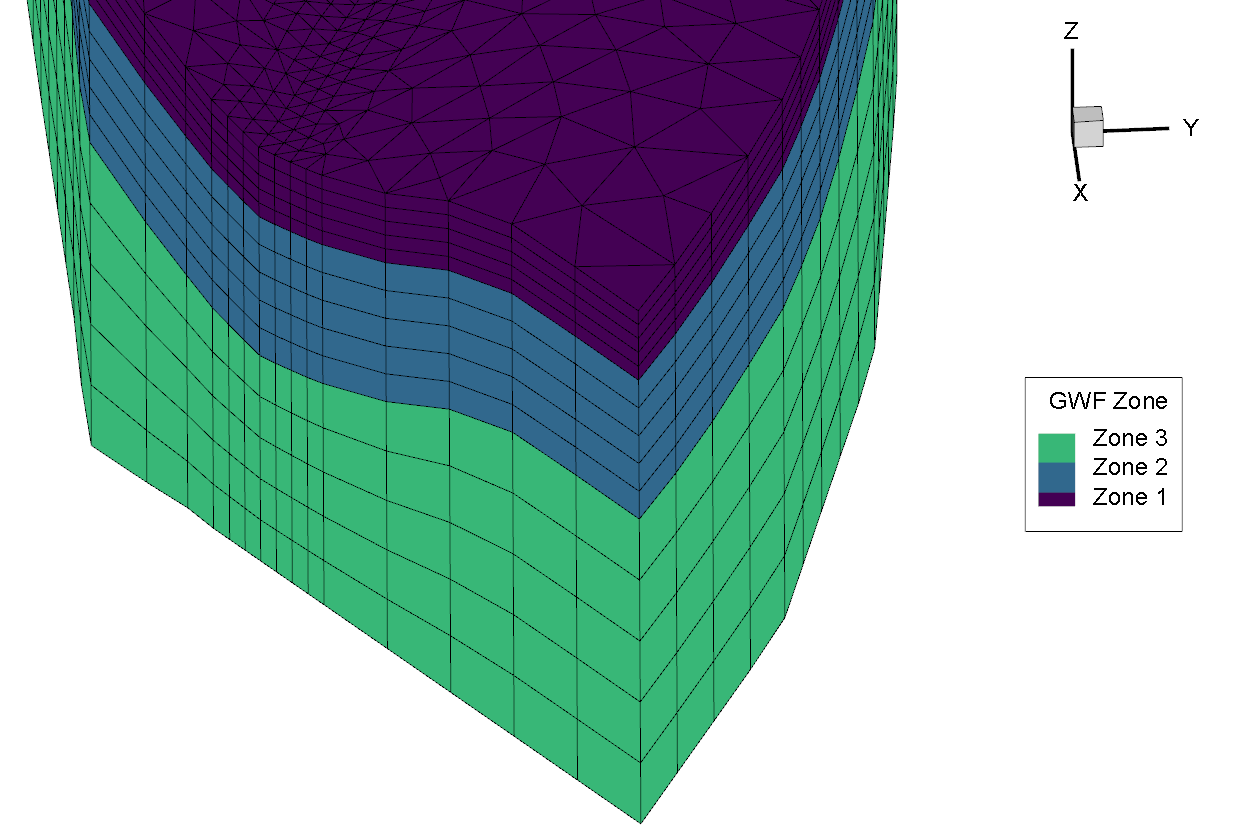
\includegraphics[width=.86\textwidth]{3_10_GWFZones}

\pagebreak
Some key features to note are:
\begin{itemize}
    \item There are 3 zones, corresponding to the layers 1 to 3.
    \item 'Zone 1', coloured dark blue, corresponds to layer 1.  Recall that the \mfus\ mesh is generated from the top down, so layer 1 is at the top of the model domain.
    \item Each layer is composed of multiple \mf\ layers, which are each one cell thick.
\end{itemize}

The following example uses the materials database and zone selection to assign material properties for the 3-layer case:

\begin{verbatim}
    gwf materials database
    	Materials file C:\MUT\MUT_Examples-main\_MUT_USERBIN\qryGWFMaterials.txt

    active domain
    	gwf

    clear chosen zones
    	GWF Zones chosen:          0

    choose zone number
    	Adding zone number:        1
    	GWF zone numbers currently chosen:
    	    1

    choose zone number
    	Adding zone number:        2
    	GWF zone numbers currently chosen:
    	    1
    	    2

    choose zone number
    	Adding zone number:        3
    	GWF zone numbers currently chosen:
    	    1
    	    2
    	    3

    clear chosen cells
    	GWF Cells chosen:          0

    choose cells by chosen zones
    	GWF Cells chosen:      39765

    chosen cells use gwf material number
    	Assigning all chosen GWF cells properties of material               4, Borden sand
    	Kh_Kx:                 1.00000E-05
    	Kv_Kz:                 1.00000E-05
    	Specific Storage:      1.20000E-07
    	Specific Yield:        0.34000
    	Alpha:                  1.9000
    	Beta:                   6.0000
    	Sr:                    0.18000
    	Unsaturated Function Type:   Van Genuchten
\end{verbatim}

Some key features to note are:
\begin{itemize}
    \item As we choose zone numbers, the list of currently chosen zones grows accordingly.
    \item The final number of \gwf\ cells chosen is equal to the total number of cells in the domain, since we had selected all 3 layers prior to converting the  zone selection to a cell selection.
    \item After assignment, the \gwf\ material number, name and assigned property values are echoed to screen and \texttt{.eco} file.
\end{itemize}

\subsubsection{Initial Conditions}  \index{\gwf\ Domain ! initial condition ! initial (starting) head}
An initial (or starting) head should be assigned to each cell in the \gwf\ domain.  This could be an initial guess at the beginning of a transient stress period or a set of hydraulic heads from a previous run.

To assign a uniform hydraulic head to the \gwf\ model domain, you must first make a cell selection as described on page~\pageref{page:cellSelect}, then use this instruction:

\ins{gwf initial head}
    {
        \squish
        \begin{enumerate}
        \item \rnum{value}  Initial (or starting) hydraulic head [L].
        \end{enumerate}
          An initial hydraulic head  of \rnum{value} is assigned to the chosen cells.
    }

To assign a linearly varying head that is a function of $z$ (i.e.\ depth or elevation), use this instruction:
\ins{gwf initial head function of z}
    {
    \squish
    \begin{enumerate}
    \item \rnum{z(1)}, \rnum{head(1)}  First $z, head$ pair.
    \item \rnum{z(2)}, \rnum{head(2)}  Second $z, head$ pair.
    \item \textbf{...}
    \item \rnum{z(n)}, \rnum{head(n)}  nth $z, head$  pair.
    \end{enumerate}

     An initial head is calculated for each chosen cell, based on it's $z$-coordinate location, by interpolating a head from the given list of  $z, head$ pairs.

     This subtask reads a list of $z, head$ pairs until an \textsf{end} instruction is encountered e.g.\:

    {\Large \sf end gwf initial head function of z}
    }

This is commonly used to generate an initial head for a simple column model \footnote{The verification example \texttt{MUT\_Examples$\backslash$1\_VSF\_Column} uses the \texttt{gwf initial head function of z} instruction to define the initial head of the model domain} as shown here: :
\begin{verbatim}
    gwf initial head function of z
    !  z    head
      0.0  -100.0
    100.0     0.0
\end{verbatim}
Some key features of this example are:
\begin{itemize}
  \item The two given $z,head$ pairs define an initial head  that varies from $head=-100.0$ at $z=0$ to $head=0.0$ at $z=100.0$.  You may supply as many pairs as needed to define the initial head.
  \item $z$-coordinates must increase continuously from the top of the list to the bottom.
  \item the $z$-range of the supplied pairs should cover the entire $z$-range of the model domain.
  \item For each node in the model domain  mesh, the $z$ coordinate is used to interpolate an initial head (i.e. $head$ value) using the appropriate $z, head$ pair.
\end{itemize}

\subsubsection{Boundary Conditions}  \index{\gwf\ Domain ! boundary conditions}
A constant head boundary condition fixes the head at a \gwf\ cell at a given value, allowing water to flow into or out of the \gwf\ model domain depending on surrounding conditions.    To assign a uniform constant head to the \gwf\ model domain use this instruction:

\ins{gwf constant head}
    {
        \squish
        \begin{enumerate}
        \item \rnum{value}  Constant hydraulic head [L].
        \end{enumerate}
          An constant hydraulic head  of \rnum{value} is assigned to the chosen cells.
    }

A drain boundary condition allows water to flow out of the \gwf\ model domain if the hydraulic head of the cell is higher than the drain elevation.   To add a drain to the \gwf\ model domain use this instruction:

\ins{gwf drain}
    {
        \squish
        \begin{enumerate}
        \item \rnum{value}  Drain conductance [L/T].
        \end{enumerate}
          A drain conductance of \rnum{value} is assigned to the chosen cells.  The top elevation of the cell is assigned automatically as the drain elevation
    }

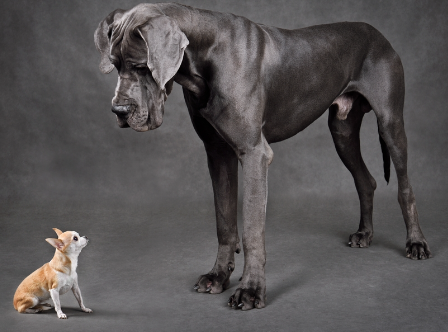
\includegraphics[width=.15\textwidth]{ModelDevelopment} \textit{Should we add an instruction where the drain elevation is specified?  }

A recharge boundary condition forces  water to flow in to the \gwf\ model domain at a specified rate.   To add a recharge  to the \gwf\ model domain use this instruction:

\ins{gwf recharge}
    {
        \squish
        \begin{enumerate}
            \item \rnum{value}  Recharge rate [L/T].
            \item \inum{option}  Recharge option.
        \end{enumerate}
        A recharge rate of \rnum{value} is assigned to the chosen cells.

        The recharge option \inum{option}is used to define where the recharge  is to be applied and can have one of the following values:
        \begin{enumerate}
            \item To top layer
            \item To one specified node in each vertical column
            \item To highest active node in each vertical column
            \item To the swf domain on top of each vertical column
        \end{enumerate}
        \squish
    }

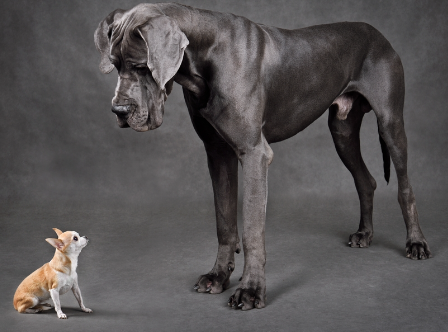
\includegraphics[width=.15\textwidth]{ModelDevelopment} \textit{Sould we have an example of pumping with an assigned nodal flux?  Should it be from a CLN?  Is there a boundary condition that assures the head will not be drawn down below the pumping node elevation?}






    \section{Surface Water Flow(\swf) Domain} \label{texfile:SWF}
The \swf\ domain is a 2D network of cells which is usually, but not necessarily, coincident with the top of the \gwf\ domain.

\mfus\ allows individual (i.e.\ \gwf, \swf\ and \cln)  processes  to add to the global
conductance matrix in order to represent fluxes between cells
within a process as well as with cells of other processes.
\mfus\ provides a framework for tightly
coupling multiple hydrologic processes. The tight coupling, in
contrast to a sequential or iterative coupling approach, occurs
through the formulation of a global conductance matrix that
includes the cells for all processes.

The flows between \swf\ cells are governed by the diffusion-wave equations, which ultimately provide a pressure head (i.e. surface water depth) at each cell.

\subsection{Generating a \swf\ Domain}
A \swf\ domain can be easily added to the \mfus\ model using the same template mesh that was used to define the \gwf\ mesh, as described in Section~\ref{texfile:TemplateMesh}.

The \swf\ domain is generated using this instruction:

\ins{generate swf domain}
    {This subtask currently has only one instruction that is used to define:
     \begin{itemize}
        \item Top elevation (e.g.\ ground surface elevation)
    \end{itemize}

    An end instruction is required to stop the subtask e.g.:

    {\Large \sf end generate swf domain}
    }

Here, the \textsf{top elevation} instruction has the same options as described in Section~\ref{section:topelev} for the \gwf\ domain.

Currently, the element zone numbering for the \swf\ domain is determined by the instruction used to generate the template mesh:
\begin{description}
  \item[2d mesh from gb] The \gb\ element area numbers are used to define the \mfus\ element zone numbers.
  \item[generate uniform rectangles] The element zone numbers default to 1.
\end{description}

%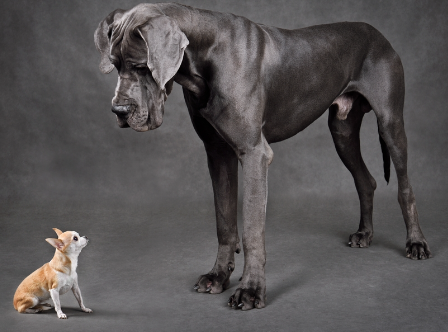
\includegraphics[width=.15\textwidth]{ModelDevelopment} \textit{We should provide instructions for defining swf zone numbers, e.g.\ from a cell list or raster file.}

\subsubsection{Cell Connection Properties}  \index{\swf\ Domain ! cell connection properties}

The \swf-\swf\ lateral cell connection lengths and areas are defined in the same way as they are for the \gwf\ domain (see Section~\ref{section:GWFCellConnections}), except lateral connection area uses surface water depth instead of cell thickness.

\swf-\gwf\ cell connection properties vary on a cell-by-cell basis:
\begin{itemize}
     \item By default, the \swf-\gwf\ connection length is assigned a value of 0.001.
     \item The vertical \swf-\gwf\ connection area is defined in the same way as it is for vertical \gwf-\gwf\ cell connections (see Section~\ref{section:GWFCellConnections}).
\end{itemize}

You can use this instruction to change the \swf-\gwf\ cell connection length after making a cell selection (see the instructions described on page~\pageref{page:cellSelect} for the \gwf\ domain):

\ins{swf to gwf connection length}
    {
        \squish
        \begin{enumerate}
        \item \rnum{Sgcl} [$L$] \swf\ cell to \gwf\ cell connection length.
        \end{enumerate}
          A \swf\ cell to \gwf\ cell connection length \rnum{Sgcl} is assigned to the chosen cells.
    }

\subsubsection{Material Properties}  \index{\swf\ Domain ! material properties}
Unlike the \gwf\ domain, \swf\ domain material properties vary on a zone-by-zone basis, which means assigning material property values are done using zone selections instead of cell selections.

%\swf\ material properties that vary on a zone-by-zone basis are:
%\begin{itemize}
%     \item Manning's coefficient of friction.
%     \item Depression storage height.
%     \item Obstruction storage height.
%     \item \swf\ depth for smoothing (h1 and h2)
%\end{itemize}
%
Prior to making zone selections and assigning properties, we need to activate the \swf\ domain using these instructions:
\begin{verbatim}
    active domain
    swf
\end{verbatim}

Zone selections must first be made using the instructions described on page~\pageref{page:zoneSelect} for the \gwf\ domain, then these instructions can be used to assign material properties to the current zone selection:

\ins{swf manning}
    {
        \squish
        \begin{enumerate}
        \item \rnum{Manning} [$L^{-1/3}$  $T$].  Manning's coefficient of friction
        \end{enumerate}
          A Manning's coefficient of \rnum{Manning} is assigned to the chosen cells.
    }

\ins{swf depression storage height}
    {
        \squish
        \begin{enumerate}
        \item \rnum{DHeight} [$L$]  Depression storage height.
        \end{enumerate}
          A depression storage height of \rnum{DHeight} is assigned to the chosen zones.
    }

\ins{swf obstruction storage height}
    {
        \squish
        \begin{enumerate}
        \item \rnum{OHeight} [$L$]  Obstruction storage height.
        \end{enumerate}
          An obstruction storage height of \rnum{OHeight} is assigned to the chosen zones.
    }

\ins{swf depth for smoothing}
    {
        \squish
        \begin{enumerate}
        \item \rnum{Depth1} [$L$]  Depth for smoothing height 1.
        \item \rnum{Depth2} [$L$]  Depth for smoothing height 2.
        \end{enumerate}
          Two depth for smoothing heights are read in \rnum{Depth1} and \rnum{Depth2} and assigned to the chosen zones.
    }

A lookup table of \swf\ material properties  is provided in the file \texttt{SWF.csv}, located in the \bin\ directory as outlined on page~\pageref{page:userbin}.

In order for \mut\ to access the lookup table, you first need to provide a link to this file using the instruction:

\ins{swf materials database}
    {
        \squish
        \begin{enumerate}
        \item \str{FName}  \swf\ material properties lookup table file name.
        \end{enumerate}
          \mut\ uses the file \str{FName} to look up \swf\ material properties.
    }

You can now assign a full set of \swf\ material properties to the current zone selection, as described on page~\pageref{page:zoneSelect}, using this instruction:

\ins{chosen zones use swf material number}
    {
        \squish
        \begin{enumerate}
        \item \inum{MaterialID}  \swf\ material ID number.
        \end{enumerate}
        The unique set of \swf\ material properties with ID number \inum{MaterialID} is retrieved from the lookup table and assigned to the chosen cells.    }

The assigned \swf\ material properties are written to the screen and \texttt{.eco} file e.g.:
\begin{verbatim}
    chosen zones use swf material number
    	Assigning all chosen SWF zones properties of material     4, Grass
    	Manning's Coefficient:          0.30000         METERS^(-1/3)  SECONDS
    	Depression Storage Height:      0.10000         METERS
    	Obstruction Storage Height:      0.0000         METERS
    	SWF Smoothing Depth 1:          1.00000E-06     METERS
    	SWF Smoothing Depth 2:          1.00000E-06     METERS
\end{verbatim}

You can find detailed information about how to use \excel\ to modify or define your own lookup tables in Appendix~\ref{Appendix:ExcelUseage}.

\subsubsection{Initial Conditions}  \index{\swf\ Domain ! initial condition ! initial (starting) depth}
An initial (or starting) head should be assigned to each cell in the \swf\ domain.  This could be an initial guess at the beginning of a transient stress period or a set of hydraulic heads from a previous run.

To assign an initial head to the \swf\ model domain, you must first make a cell selection as described on page~\pageref{page:cellSelect}, then this instruction can be used to calculate an initial (or starting) head for the flow solution given an initial surface water depth:

\ins{swf initial depth}
    {
        \squish
        \begin{enumerate}
        \item \rnum{IDepth} [$L$]  Initial depth.
        \end{enumerate}
          An initial depth of \rnum{IDepth} is used to calculate an initial head at each of the chosen cells.
    }

\subsubsection{Boundary Conditions}  \index{\swf\ Domain ! boundary conditions}
To assign boundary conditions  to the \swf\ model domain, you must first make a cell selection as described on page~\pageref{page:cellSelect}.

A constant head boundary condition fixes the head at a \swf\ cell at a given value, allowing water to flow into or out of the \swf\ model domain depending on surrounding conditions.    To assign a uniform constant head to the \swf\ model domain use this instruction:

\ins{swf constant head}
    {
        \squish
        \begin{enumerate}
        \item \rnum{CHead} [$L$]  Constant hydraulic head.
        \end{enumerate}
          An constant hydraulic head  of \rnum{CHead} is assigned to the chosen cells.
    }

A recharge boundary condition forces  water to flow in to the \swf\ model domain at a specified rate.   To add recharge  to the \swf\ model domain use this instruction:

\ins{swf recharge}
    {
        \squish
        \begin{enumerate}
            \item \rnum{RechRate} [$L$ $T^{-1}$] Recharge rate.
            \item \inum{RechOpt}  Recharge option.
        \end{enumerate}
        A recharge rate of \rnum{RechRate} is assigned to the chosen cells.

        The recharge option \inum{RechOpt} is used to define where the recharge is to be applied and in this case should be set to a value of 4, which applies the recharge to the \swf\ domain.
    }

A well boundary condition forces  water to flow in or out of the \swf\ model domain at a specified rate.   To add a well  to the \swf\ model domain use this instruction:

\ins{swf well}
    {
        \squish
        \begin{enumerate}
            \item \rnum{PumpRate} [$L^{3}$ $T^{-1}$]  Pumping rate.
        \end{enumerate}
        A pumping  rate of \rnum{PumpRate} is assigned to the chosen cells.  Positive pumping rates add water to the domain, negative pumping rates remove water from the domain.
    }

A critical depth boundary condition assigned to a \swf\ cell allows water to flow out of the \swf\ model domain at a rate that depends on the surface water depth and a contributing length (i.e.\ representing the length of the cell side over which the outflow occurs).

\pagebreak
One of the following two  instructions can be used to assign a critical depth outflow boundary condition to the \swf\ model domain:

\ins{swf critical depth with sidelength1}
    {
          A critical depth outflow boundary condition is assigned to the chosen cells.

          It is assumed that an accurate estimate of the contributing length of a cell can be based on the square root of the cells horizontal area.
    }


\ins{swf critical depth}
    {
          A critical depth outflow boundary condition is assigned to the chosen cells.

          The contributing length of the cell outflow boundary is calculated from the \swf\ mesh outer boundary nodes, with each outer boundary node connected to a chosen cell contributing a half-element side length in both directions along the outer boundary.
    }

Although \textsf{swf critical depth} is less convenient than \textsf{swf critical depth with sidelength1}, it does calculate a contributing length that matches the actual length along the \swf\ mesh outer boundary.

The example \texttt{6\_Abdul\_Prism\_Cell} uses the second approach to define the critical depth outflow boundary condition:
\begin{verbatim}
        clear chosen nodes
        choose gb nodes
        ./gb/grid.nchos.Outer boundary nodes
        flag chosen nodes as outer boundary

        clear chosen cells
        clear chosen nodes
        choose cells from gb elements
        ./gb/grid.echos.Critical depth outlet
        swf critical depth
\end{verbatim}

Some key features of this example are:
\begin{itemize}
    \item \swf\ {\em nodes} are chosen and flagged to be on the outer boundary with the instruction \textsf{flag chosen nodes as outer boundary}.
    \item \swf\ {\em cells} are chosen using a \gb\ chosen {\em elements} file with the instruction \textsf{choose cells from gb elements}.  Because this example was generated using the mesh-centred control volume approach, there is a 1-to-1 correspondence between template mesh elements and \swf\ cells.

        In the example \texttt{6\_Abdul\_Prism\_Cell\_nc}, the node-centred control volume approach is used and the instruction \textsf{choose cells from gb nodes} is used instead, because in this case there is a 1-to-1 correspondence between template mesh {\em nodes} and \swf\ cells.
\end{itemize}

The \swf\ and \gwf\ meshes that \mut\ generates inherit node and element information from the template mesh.  Currently, you can define node selections using these instructions: \label{page:nodeSelect}

\ins{choose all nodes}
    {Select all nodes in the active model domain.
     }

\ins{choose node at xyz}
    {
        \squish
        \begin{enumerate}
        \item \rnum{x1} [$L$], \rnum{y1} [$L$], \rnum{z1} [$L$]  An $xyz$ coordinate triplet.
        \end{enumerate}
        The node closest to the given $xyz$ coordinate triplet will be chosen.
    }

\ins{choose gb nodes}
    {
        \squish
        \begin{enumerate}
        \item \str{FName}  The \gb\ chosen node \str{FName} containing information concerning the status, chosen or not chosen, of each node in the \gb\ model domain.
        \end{enumerate}
          If a node is flagged as chosen in the \gb\ model domain then the corresponding node will be chosen in the \mfus\ model domain.
    }

\ins{clear chosen nodes}
    {Clears the current node selection.
     }



    \section{Connected Linear Network(\cln ) Domain} \label{texfile:CLN}
A \cln\ domain is a quasi-3D network of modflow cells which are each defined by individual line segments. The flows between \cln\ cells are governed by either open- or closed-channel flow equations, depending on surrounding conditions, which ultimately provide a pressure head or water depth at each cell.

\mut\ adds the \cln\ process equations to the global
conductance matrix in order to represent fluxes between cells
within the process as well as with cells of other processes.

The current version of \mut\ has the following limitations for the definition of the \cln\ domain:
\begin{enumerate}
    \item General \cln\ domains, where the cell geometry is independent of the \gwf\ mesh and  cell-to-cell connection can be one-to-many or many-to-one are not yet implemented. \mut\ assumes a 1-to-1 connection exists between \cln\ cells and \gwf\ layer 1 cells (i.e. top layer).
    \item \cln\ flows to the \gwf\ domain are implemented, but not  \cln\ flows to the \swf\ domain.
\end{enumerate}

This is sufficient for the short-term purpose of solving the example \texttt{3\_1\_CLN\_for\_SWF}, which compares the use of a \cln\ versus an \swf\ domain for simulating flow in a surface water domain coupled to a \gwf\ domain, but not for solving more general problems of interest.

\subsection{Generating a \cln\ Domain}
A \cln\ domain can be added to the \mfus\ model using this instruction:

\ins{generate cln domain}
    {This subtask is currently limited to defining the \cln\ domain from a single pair of $xyz$ coordinates and a specified number of cells.

    An end instruction is required to stop the subtask e.g.:
    
    {\Large \sf end generate cln domain}
    }

This instruction can be used to define a simple \cln\ domain:

\ins{cln from xyz pair}
    {
        \squish
        \begin{enumerate}
        \item \rnum{x1} [$L$], \rnum{y1} [$L$], \rnum{z1} [$L$]  First $xyz$ coordinate triplet.
        \item \rnum{x2} [$L$], \rnum{y2} [$L$], \rnum{z2} [$L$]  Second $xyz$ coordinate triplet.
        \item \inum{nCells}  Number of cells in the \cln.
        \end{enumerate}
        The 2 given $xyz$ coordinates define the endpoints of a line defining the \cln.  The \cln\ is subdivided into \inum{nCells} individual cells.
    }

In the example \texttt{3\_1\_CLN\_for\_SWF}, the inputs are defined so the \cln\ cells coincide exactly with the top layer of \gwf\ cells as shown below:
\begin{verbatim}
    generate uniform rectangles
    101.0, 101, -0.5   !  Mesh length in X, nRectElements in X, X Offset
    1.0, 1, -0.5   !  Mesh length in Y, nRectElements in Y, Y Offset


    generate layered gwf domain

        top elevation
            elevation from xz pairs
                 -100.0,  3.0
                  200.0,  0.0
            end elevation from xz pairs
        end top elevation

        new layer
            layer name
            Top layer

            uniform sublayering
            1

            elevation from xz pairs
                 -100.0,  2.0
                  200.0, -1.0
            end elevation from xz pairs
        end new layer

    end generate layered gwf domain

    generate cln domain
        cln from xyz pair
              -.5    0.0     2.005
            100.5    0.0     0.995
            101  ! number of new CLN cells

    end generate cln domain

\end{verbatim}

Some key features of this example are:
\begin{itemize}
    \item A template mesh of length 101.0 and with 101 elements is used to define the \gwf\ domain.
    \item The mesh is offset in $x$ by -0.5 m so that \gwf\ and \cln\ cell locations start at $x=0.0$ and end at $x=100$ m.
    \item The top of the \gwf\ domain slopes from $z=3.0$ at $x=-100.0$ to $z=0.0$ at $x=200.0$.  These are extended beyond the limits of the mesh so that the correct elevations are generated at the limits of the domain. Recall that the $x$-range must cover the entire template mesh.
    \item Because \cln\ domains are not necessarily dependent on \gwf\ meshes, it does not use the template mesh, but instead generates a \cln\ domain using the  \texttt{cln from xyz pair} instruction.  The instruction is set up to generate 101 \cln\ cells that slope from $z=2.005$ at $x=-.5$ to $z=0.995$ at $x=100.5$
\end{itemize}

\subsubsection{Cell Connection Properties}  \index{\cln\ Domain ! cell connection properties}

\cln\ domain cells are currently limited to have a direct one-to-one correspondence with cells in the top layer of the \gwf\ domain, as is the case for the simple example \texttt{3\_1\_CLN\_for\_SWF}.  A more general approach, in which \cln\ cells do not have to conform to the \gwf\ or \swf\ meshes will be developed in a subsequent version of \mut.

\cln-\cln\ cells are connected through neighbouring nodes and connection properties are defined by the channel geometry inputs.

\cln-\gwf\ cell vertical connections are defined by element areas.

\subsubsection{Material Properties}  \index{\cln\ Domain ! material properties}
\cln\ domain material properties vary on a zone-by-zone basis.  In the current version of \mut\, the assignment of \cln\ material properties is very rudimentary.

Prior to assigning properties, we need to activate the \cln\ domain using these instructions:
\begin{verbatim}
    active domain
    cln
\end{verbatim}

A lookup table of \cln\ material properties  is provided in the file \texttt{CLN.csv}, located in the \bin\ directory as outlined on page~\pageref{page:userbin}.

In order for \mut\ to access the lookup table, you first need to provide a link to this file using the instruction:

\ins{cln materials database}
    {
        \squish
        \begin{enumerate}
        \item \str{FName}  \cln\ material properties lookup table file name.
        \end{enumerate}
          \mut\ uses the file \str{FName} to look up \cln\ material properties.
    }

Zone selections must first be made using the instructions described on page~\pageref{page:zoneSelect} for the \gwf\ domain.

You can now assign a full set of \cln\ material properties to the current zone selection, as described on page~\pageref{page:zoneSelect}, using this instruction:

\ins{chosen zones use cln material number}
    {
        \squish
        \begin{enumerate}
        \item \inum{MaterialID}  \cln\ material ID number.
        \end{enumerate}
        The unique set of \cln\ material properties with ID number \inum{MaterialID} is retrieved from the lookup table and assigned to the chosen cells.    }

The assigned \cln\ material properties are written to the screen and \texttt{.eco} file:
\begin{verbatim}
    chosen zones use cln material number
    	Assigning all chosen CLN zones properties of material 1, 2D Hillslope 100 m length
    	Geometry:           Rectangular
    	Rectangular Width:       1.0000         METERS
    	Rectangular Height:      1.0000         METERS
    	Direction:          Horizontal
    	Flow Treatment:     Unconfined/Mannings
    	Longitudinal K:         5.48000E-02     METERS   SECONDS^(-1)
\end{verbatim}

You can find detailed information about how to use \dbase\ to modify or define your own lookup tables in Tutorial~\ref{Appendix:ExcelUseage}.

\subsubsection{Initial Conditions}  \index{\cln\ Domain ! initial condition ! initial (starting) depth}
An initial (or starting) head should be assigned to each cell in the \cln\ domain.  This could be an initial guess at the beginning of a transient stress period or a set of hydraulic heads from a previous run.

To assign an initial head to the \cln\ model domain, you must first make a cell selection as described on page~\pageref{page:cellSelect}, then this instruction can be used to calculate an initial (or starting) head for the flow solution given an initial water depth:

\ins{cln initial depth}
    {
        \squish
        \begin{enumerate}
        \item \rnum{Depth} [$L$]  Initial depth.
        \end{enumerate}
          An initial depth of \rnum{Depth} is used to calculate an initial head at each of the chosen cells.
    }

\subsubsection{Boundary Conditions}  \index{\cln\ Domain ! boundary conditions}
To assign boundary conditions  to the \cln\ model domain, you must first make a cell selection as described on page~\pageref{page:cellSelect}.

A constant head boundary condition fixes the head at a \cln\ cell at a given value, allowing water to flow into or out of the \cln\ model domain depending on surrounding conditions.    To assign a uniform constant head to the \cln\ model domain use this instruction:

\ins{cln constant head}
    {
        \squish
        \begin{enumerate}
        \item \rnum{CHead} [$L$]  Constant hydraulic head.
        \end{enumerate}
          An constant hydraulic head  of \rnum{CHead} is assigned to the chosen cells.
    }

A well boundary condition forces  water to flow in or out of the \cln\ model domain at a specified rate.   To add a well  to the \cln\ model domain use this instruction:

\ins{cln well}
    {
        \squish
        \begin{enumerate}
            \item \rnum{PumpRate} [$L^{3}$ $T^{-1}$]  Pumping rate.
        \end{enumerate}
        A pumping  rate of \rnum{PumpRate} is assigned to the chosen cells. Positive pumping rates add water to the domain, negative pumping rates remove water from the domain.
    }



    \section{Stress Periods} \label{section:StressPeriods}
A \mfus\ simulation can be broken up into separate periods of time called ''stress periods''.  Boundary conditions can be defined at the beginning of each stress period and changed in subsequent stress periods.

At least one stress period must be defined using this instruction:

\ins{stress period}
    {This subtask has several instructions that can be used to define the duration, type and timestepping parameters of the stress period.

    It reads instructions until an \textsf{end} instruction is found e.g.\:

    {\Large \sf end stress period}
    }

These instructions can be used to define the stress period parameters:

\ins{type}
    {
        \squish
        \begin{enumerate}
        \item \str{type}  Stress period type.
        \end{enumerate}
        The stress period type is defined by the string \str{type}.  It can be one of the following:
        \begin{itemize}
            \item \textsf{SS} A steady-state stress period in which the simulation is carried out until it reaches a state of equilibrium with the defined boundary conditions.
            \item \textsf{TR} A transient stress period in which the simulation is carried out for a specified duration with the defined boundary conditions.
        \end{itemize}
        \squish
    }

\ins{duration}
    {
        \squish
        \begin{enumerate}
        \item \rnum{value}  Stress period duration [T].
        \end{enumerate}
        The stress period duration, is defined by the string \rnum{value}.  It should be entered using the correct units of time as outlined in Section~\ref{section:Units}.
    }

\ins{number of timesteps}
    {
        \squish
        \begin{enumerate}
        \item \inum{value}  Number of timesteps to be used for this stress period.
        \end{enumerate}
        \squish
    }

You can change the default  starting time step size of  $1\times10^{-3}$ seconds with this instruction:

\ins{deltat}
    {
        \squish
        \begin{enumerate}
        \item \rnum{value}  Starting time step size [T].
        \end{enumerate}
        The  starting time step size used for the stress period  is defined by the string \rnum{value}.  It should be entered using the correct units of time as outlined in Section~\ref{section:Units}.
    }

You can change the default  minimum time step size of  $1\times10^{-5}$ seconds with this instruction:

\ins{tminat}
    {
        \squish
        \begin{enumerate}
        \item \rnum{value}  Minimum time step size [T].
        \end{enumerate}
        The minimum time step size to allow for the stress period is defined by the string \rnum{value}.  It should be entered using the correct units of time as outlined in Section~\ref{section:Units}.
    }

You can change the default  maximum time step size of  $60.0$ seconds with this instruction:

\ins{tmaxat}
    {
        \squish
        \begin{enumerate}
        \item \rnum{value}  Maximum time step size [T].
        \end{enumerate}
        The maximum time step size to allow for the stress period is defined by the string \rnum{value}.  It should be entered using the correct units of time as outlined in Section~\ref{section:Units}.
    }


You can change the default multiplier for time step size of  $1.1$  with this instruction:

\ins{tadjat}
    {
        \squish
        \begin{enumerate}
        \item \rnum{value}  Multiplier for time step size [T].
        \end{enumerate}
        The multiplier for adjusting time step size when using adaptive time-stepping is defined by the string \rnum{value}.
    }

You can change the default divider for time step size of  $2.0$  with this instruction:

\ins{tcutat}
    {
        \squish
        \begin{enumerate}
        \item \rnum{value}  Divider for time step size [T].
        \end{enumerate}
        The divider for adjusting time step size when using adaptive time-stepping is defined by the string \rnum{value}.
    }
    
To add more stress periods, repeat the \textsf{stress period} subtask instructions and boundary condition definitions as many times as required.  Stress periods are numbered automatically as they are added.

\pagebreak
Here is an example which could be used to define two stress periods:
\begin{verbatim}
    ! stress period 1
    stress period
        type
        TR

        duration
        3000.0d0
    end stress period

    active domain
    swf
        choose all cells
        swf recharge
        5.56d-6
        4
        
        clear chosen nodes
        choose cell at xyz
        0.0 0.0 0.0 
        swf constant head
        1.0

    ! stress period 2
    stress period
        type
        TR

        duration
        3000.0d0
    end stress period

    active domain
    swf
        choose all cells
        swf recharge
        0.0d0
        4
\end{verbatim}

Some key features of this example are:
\begin{itemize}
    \item Both stress periods are transient (type TR) with a duration of 3000.
    \item The recharge applied to the \swf\ domain (recharge option 4) is 5.5e-6 for the first stress period, then is reduced to 0.0 in the second stress period.
    \item The constant head applied to the \swf\ domain in stress period 1 is maintained for the entire simulation.  By default, a boundary condition is maintained through subsequent stress periods unless it is redefined.
    \item Any boundary conditions given after an \textsf{end stress period} instruction apply to that stress period until another \textsf{stress period} instruction is encountered.
\end{itemize}


    


    \section{Output Control} \label{section:OutputControl}
This instruction can be used to generate a \mfus\ output control file:

\ins{generate output control file}
    {
    \squish
    \begin{enumerate}
    \item \rnum{t(1)}  First output time [T].
    \item \textbf{...}
    \item \rnum{t(n)}  nth output time [T].
    \end{enumerate}

          This subtask reads a list of output times \rnum{t()} until an \textsf{end} instruction is encountered e.g.\:

    {\Large \sf end generate output control file}
    }
    
The verification example \texttt{MUT\_Examples$\backslash$1\_Abdul\_prism\_cell} generates an output control file with 10 output times using these instructions:
\begin{verbatim}
    ! -----------------------------------Output Control
    generate output control file
        1e-4
        60.
        300.0
        600.0
        900.0
        1200.0
        1500.0
        3000.0
        4500.0
        6000.0
    end generate output control file
\end{verbatim}
    
The output control file looks like this:
\begin{verbatim}
    # MODFLOW-USG OC file written by Modflow-User-Tools version 1.28
    ATSA NPTIMES   10
      9.999999747378752E-005   60.0000000000000        300.000000000000
       600.000000000000        900.000000000000        1200.00000000000
       1500.00000000000        3000.00000000000        4500.00000000000
       6000.00000000000
    HEAD SAVE UNIT   114
    HEAD PRINT FORMAT 0
    DRAWDOWN SAVE UNIT   115
    DRAWDOWN PRINT FORMAT 0
    PERIOD     1
        DELTAT   1.0000E-03
        TMINAT   1.0000E-05
        TMAXAT    60.00
        TADJAT    1.100
        TCUTAT    2.000
            SAVE HEAD
            PRINT HEAD
            SAVE DRAWDOWN
            SAVE BUDGET
            PRINT BUDGET
    PERIOD     2
        DELTAT   1.0000E-03
        TMINAT   1.0000E-05
        TMAXAT    60.00
        TADJAT    1.100
        TCUTAT    2.000
            SAVE HEAD
            PRINT HEAD
            SAVE DRAWDOWN
            SAVE BUDGET
            PRINT BUDGET
\end{verbatim}

Some key features of this example are:
\begin{itemize}
    \item \mut\ automatically inserts  the  adaptive time-stepping option (\texttt{ATSA}) in the file, defines the number of print times in the simulation (NPTIMES 10) and the list of print (i.e.\ output) times.
    \item Two stress periods were defined and the listed parameters are using the default values.
\end{itemize}


    \section{Solver Parameters} \label{section:SolverParameters}
A lookup table of \mfus\ solver parameters is provided in the file \texttt{qrySMS.txt}, located in the \bin\ directory as outlined on page~\pageref{page:userbin}.

In order for \mut\ to access the lookup table, you first need to provide a link to this file using the instruction:

\ins{sms database}
    {
        \squish
        \begin{enumerate}
        \item \str{file}  Solver parameters lookup table file name.
        \end{enumerate}
          \mut\ uses the file \str{file} to look up the solver parameter values.
    }


You can find detailed information about how to use \dbase\ to modify or define your own lookup tables in Tutorial~\ref{tecfile:DbaseUseage}.

    \section{3D Model Build Visualization} \index{Model Build ! visualization}
The current version of \mut\ writes Tecplot-compatible output files that can be visualized to check the following attributes for \gwf, \swf\ and \cln\ model domains:
\begin{itemize}
  \item Finite-element mesh and \mfus\ cell locations derived from it
  \item Material properties
  \item Initial conditions
  \item Boundary conditions (if specified)
\end{itemize}

A \tecplot\ layout file, \texttt{\_build.lay}, has been created for each verification example and  provides a quick way to view the results of the model build.
We will demonstrate some basic concepts using the verification example \texttt{1\_VSF\_Column}, which has a \gwf\ domain defined by a simple 1D column mesh with boundary conditions assigned to the  top and bottom cells.

To load \texttt{\_build.lay} in \tecplot\ first navigate to the folder in File Explorer (e.g.\ \texttt{C:$\backslash$Work$\backslash$Examples$\backslash$\-1\_VSF\_Column}) then highlight the path in File Explorer:

        
\includegraphics[width=0.4\textwidth]{3_12_HighlightPath}

Replace the existing path with the string 'cmd':

        
\includegraphics[width=0.5\textwidth]{3_4_cmd}

Press Enter/Return. A command prompt window rooted at the input folder should appear. To start \tecplot\, type:
        \begin{verbatim}
            tec360
        \end{verbatim}

Choose 'Open Layout' to open a file selection dialogue:

        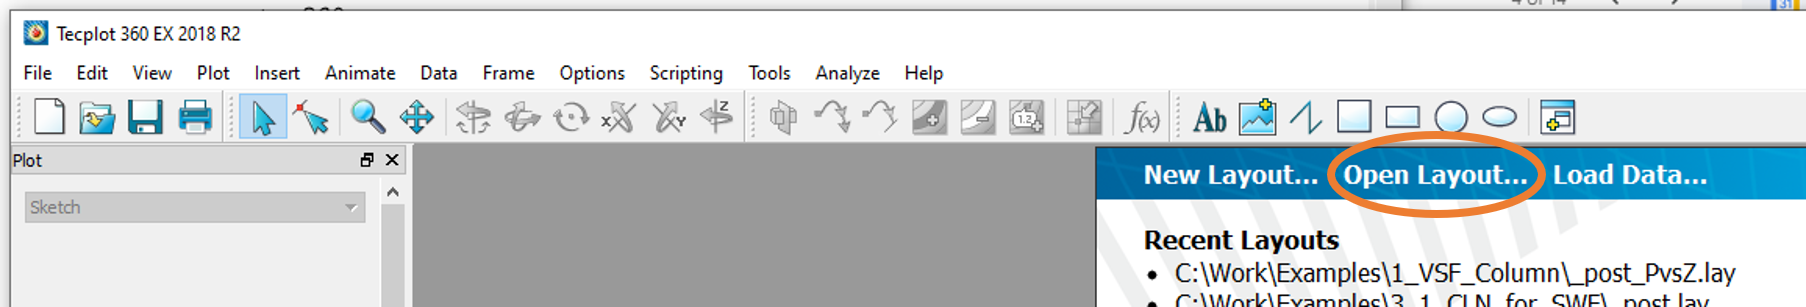
\includegraphics[width=\textwidth]{3_12_OpenLayout}

Select and open the file \texttt{\_build.lay}:

        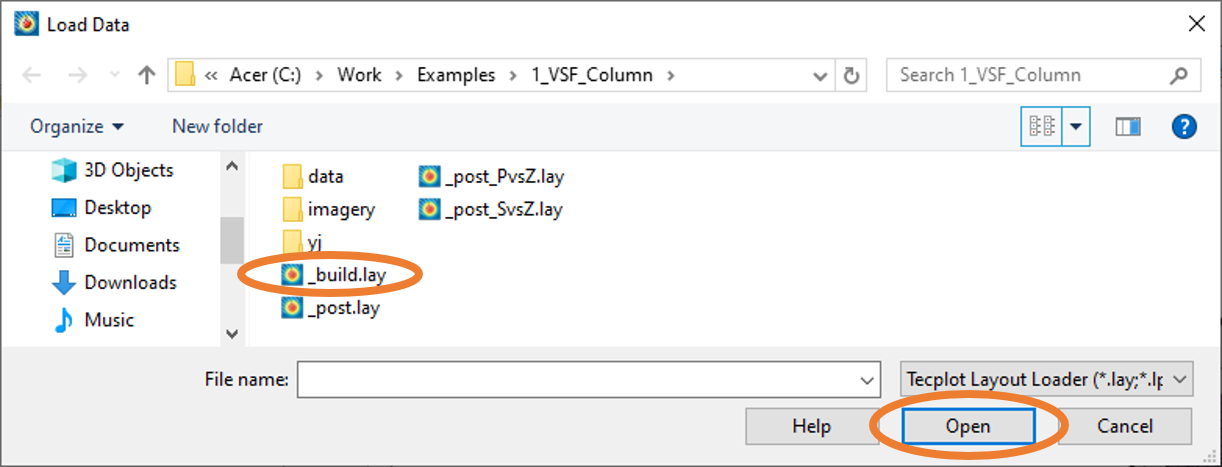
\includegraphics[width=.7\textwidth]{3_13_LayoutFiles}

You should now see the following 3D viualization of the example:

        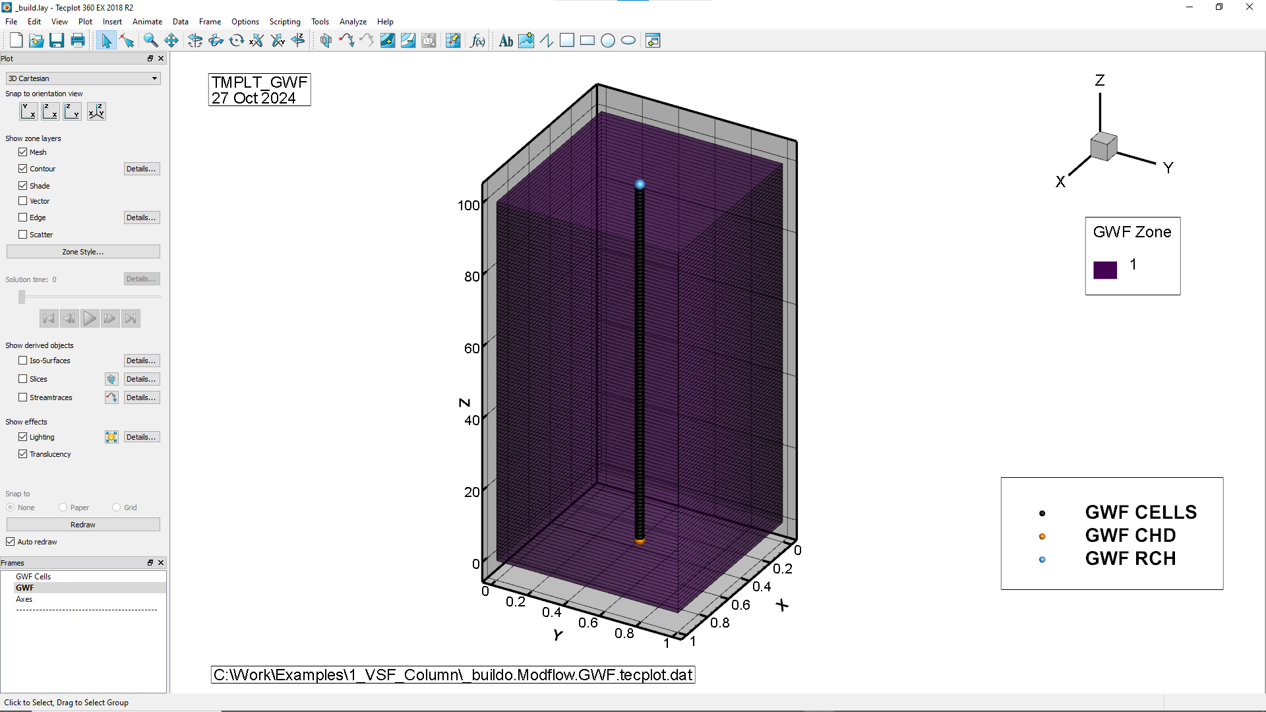
\includegraphics[width=\textwidth]{3_14_BuildLay1DColumn}

\index{\tecplot\ ! frame order}There are 4 Tecplot 'frames' that make up this image.  Each frame can house it's own data for plotting, and have unique settings for visualization.  The 'Frames' window at the bottom left corner shows the frame names and plotting order:

        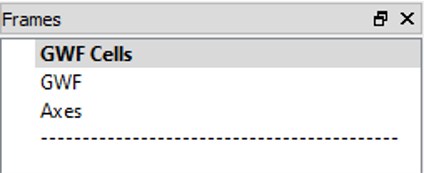
\includegraphics[width=.3\textwidth]{3_15_Frames}

The frame at the front, called \textbf{GWF Cells}, is at the top of the list, and the bold font indicates it is the currently active frame.

The frame at the bottom, indicated by the dashed line, is a special frame we will refer to as the {\sf background}.  The contents of any frame above it may be partly or completely visible, depending on which other frames are in front of it.  Move the {\sf background} to the front by right-clicking on the name and selecting 'Bring to front'.

        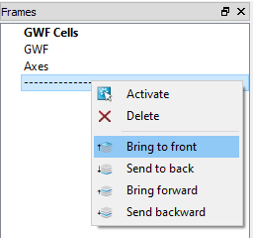
\includegraphics[width=.215\textwidth]{3_16_BringToFront}

You should now see an empty white \tecplot\ image. Right-click on the {\sf GWF} frame and bring it to the front to see it in isolation.

        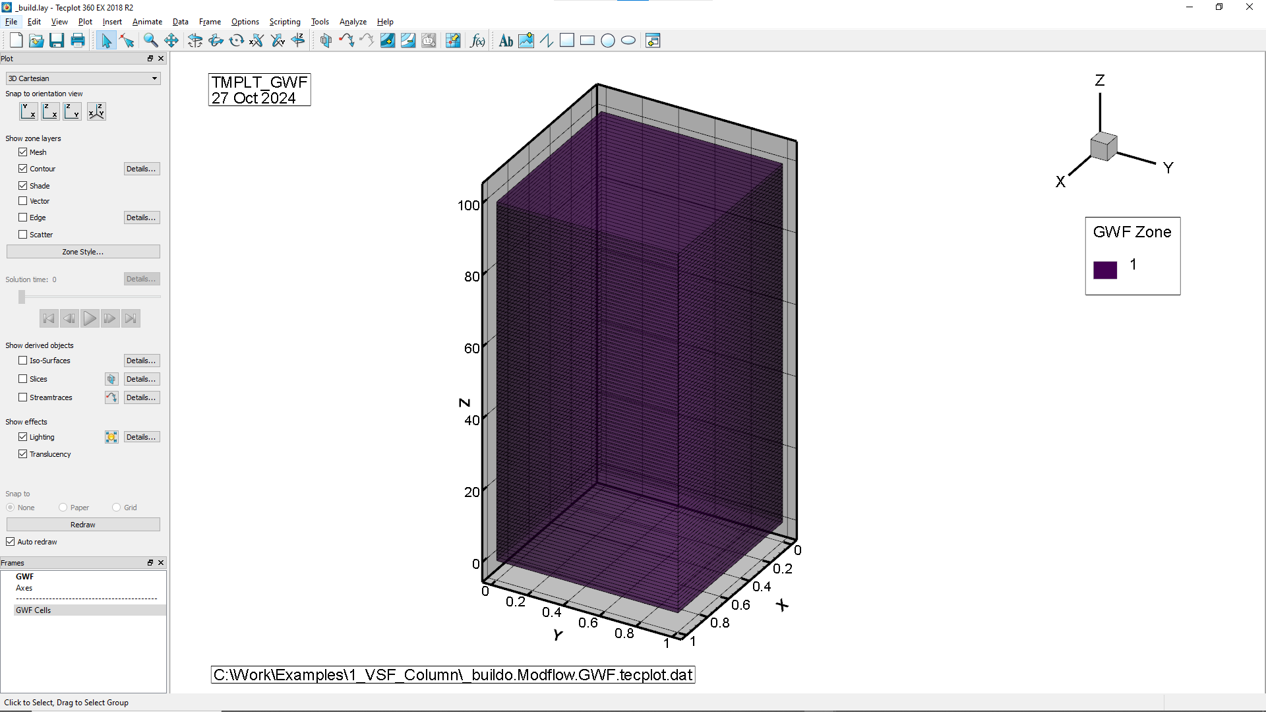
\includegraphics[width=.9\textwidth]{3_16b_GWFOnly}

Every frame below the {\sf background} frame is now invisible.

\index{\gwf\ Domain ! {\tt \_build.lay} ! {\sf GWF} frame}
The {\sf GWF} frame has the following contents:
\begin{itemize}
  \item The finite-element mesh is shown by the translucent blue-shaded volume and wireframe block elements.
  \item The names of the data files loaded into the frame are shown at the bottom left corner.
  \item The data set title and current date (on the day the file was loaded) are shown at the top left corner.  The data set title 'TMPLT\_GWF' indicates that this is the \gwf\ domain mesh that was created from the template mesh.
  \item The contouring legend, showing there is one \gwf\ zone called {\sf Zone 1}, is shown at the middle right side.
  \item The 3D orientation axis is shown at the top right corner.
\end{itemize}

Right-click on the {\sf Axes} frame and bring it to the front.

        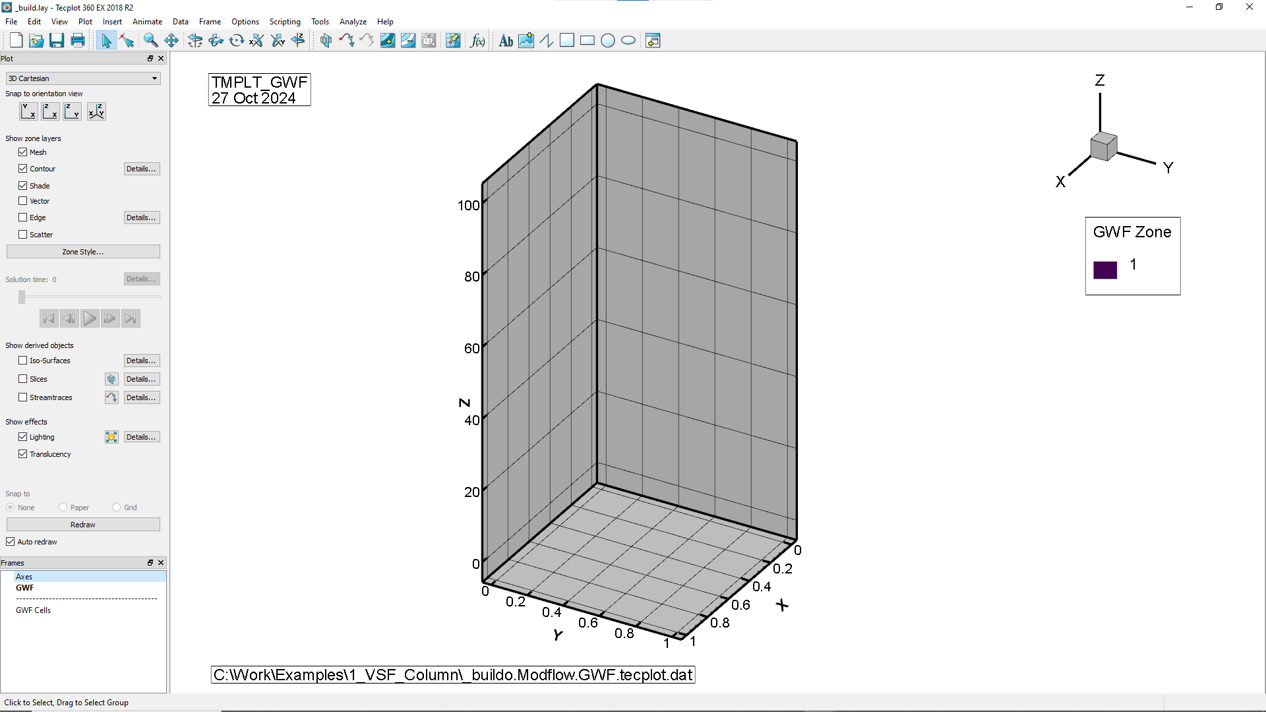
\includegraphics[width=.76\textwidth]{3_17_Axes}

Some of the contents of the {\sf GWF} frame are still visible but the finite-element mesh is obscured by the axes.  Right-click on the {\sf GWF} frame and bring it to the front.

        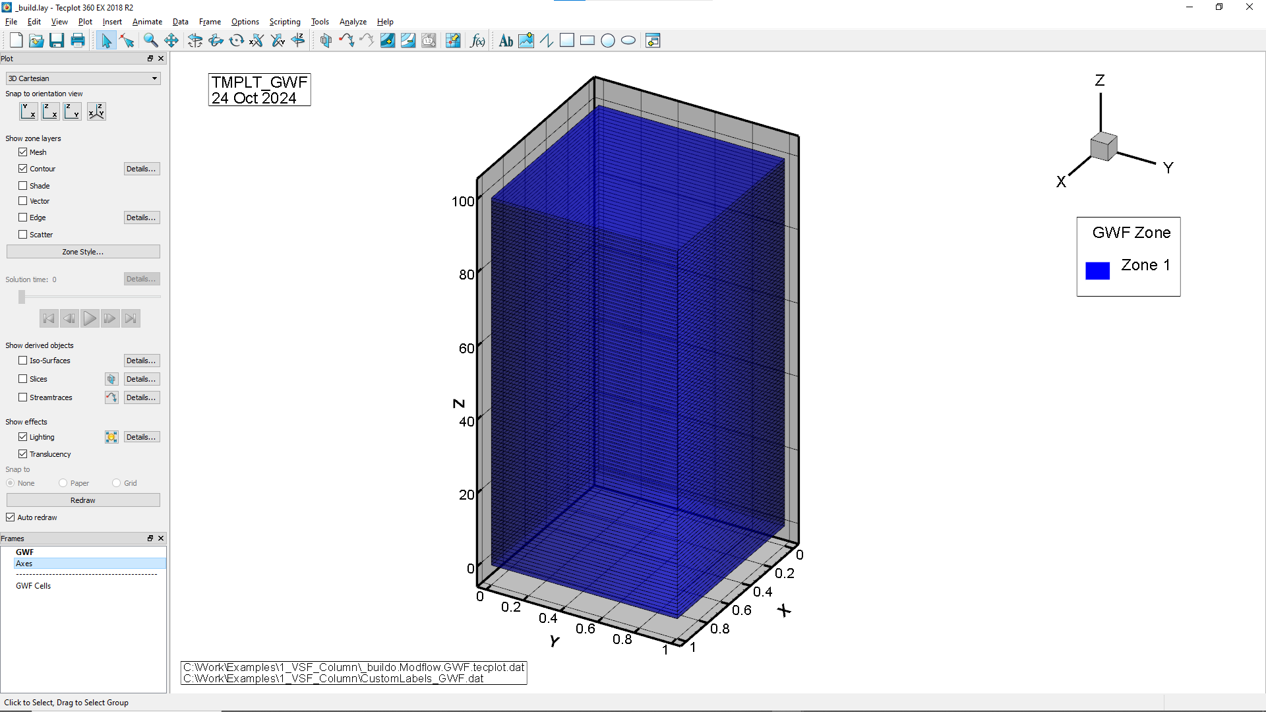
\includegraphics[width=.76\textwidth]{3_18_GWFBeforeAxes}

  The menu option {\sf Data$\backslash$Data Set Info...}(shown below left), brings up the {\sf Data Set Information} dialogue(shown below right):

        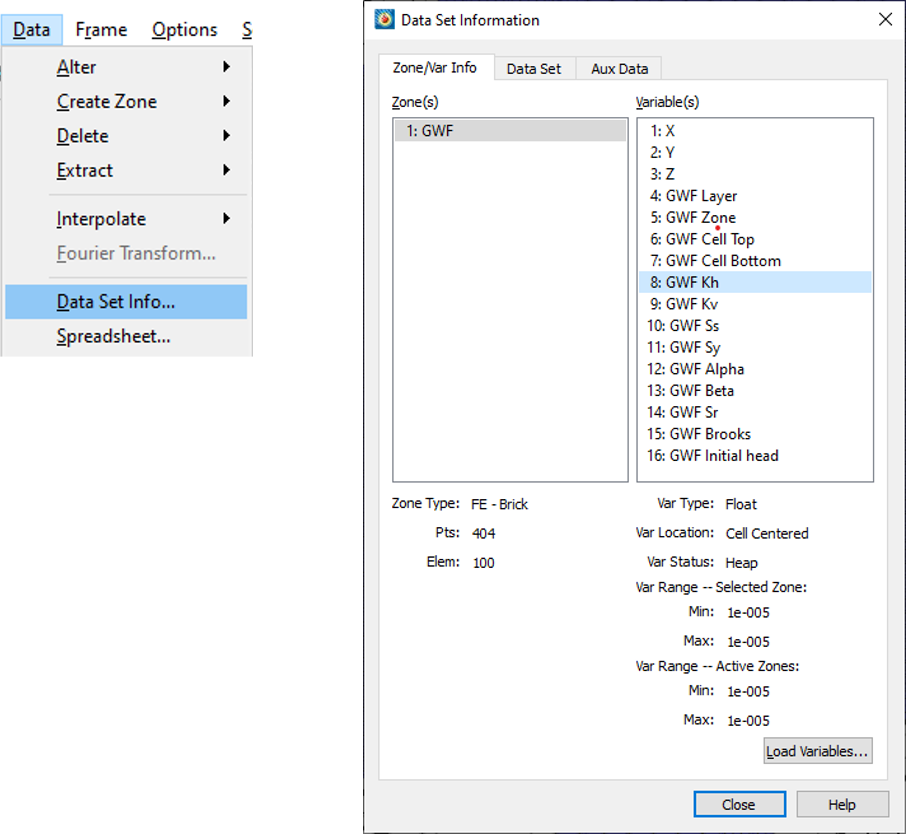
\includegraphics[width=.75\textwidth]{3_19_DataSetInfo}

The currently active frame title \gwf\ is shown in the {\sf Zone(s)} field, while the data set variables are listed in the {\sf Variable(s)} field. The variables include the $xyz$ coordinates of the {\sf TMPLT\_GWF} mesh nodes, followed by the Layer and Zone numbers assigned to the {\sf TMPLT\_GWF} mesh elements.  The remainder of the list shows the \mfus\ cell properties that were defined during the model build. The {\sf Var--Range Selected Zone:} area shows the variable {\sf Min:} and {\sf Max:} values for the currently chosen (highlighted) zone and variable (currently \gwf\ and {\sf GWF Kh} respectively).\index{\tecplot\ ! data set information}


\index{\tecplot\ ! probe tool} The \tecplot\ Probe Tool 
\includegraphics{ProbeToolButton} is used to to probe for values of the dataset's variables at a particular point. When selected, the mouse cursor changes to a modified cross-hair which indicates the Probe Tool is active. To obtain {\it interpolated} values of the dataset variables at the specified location, click at any point in the data region. 

Shown below are the results of probing the top cell of the \gwf\ domain:

        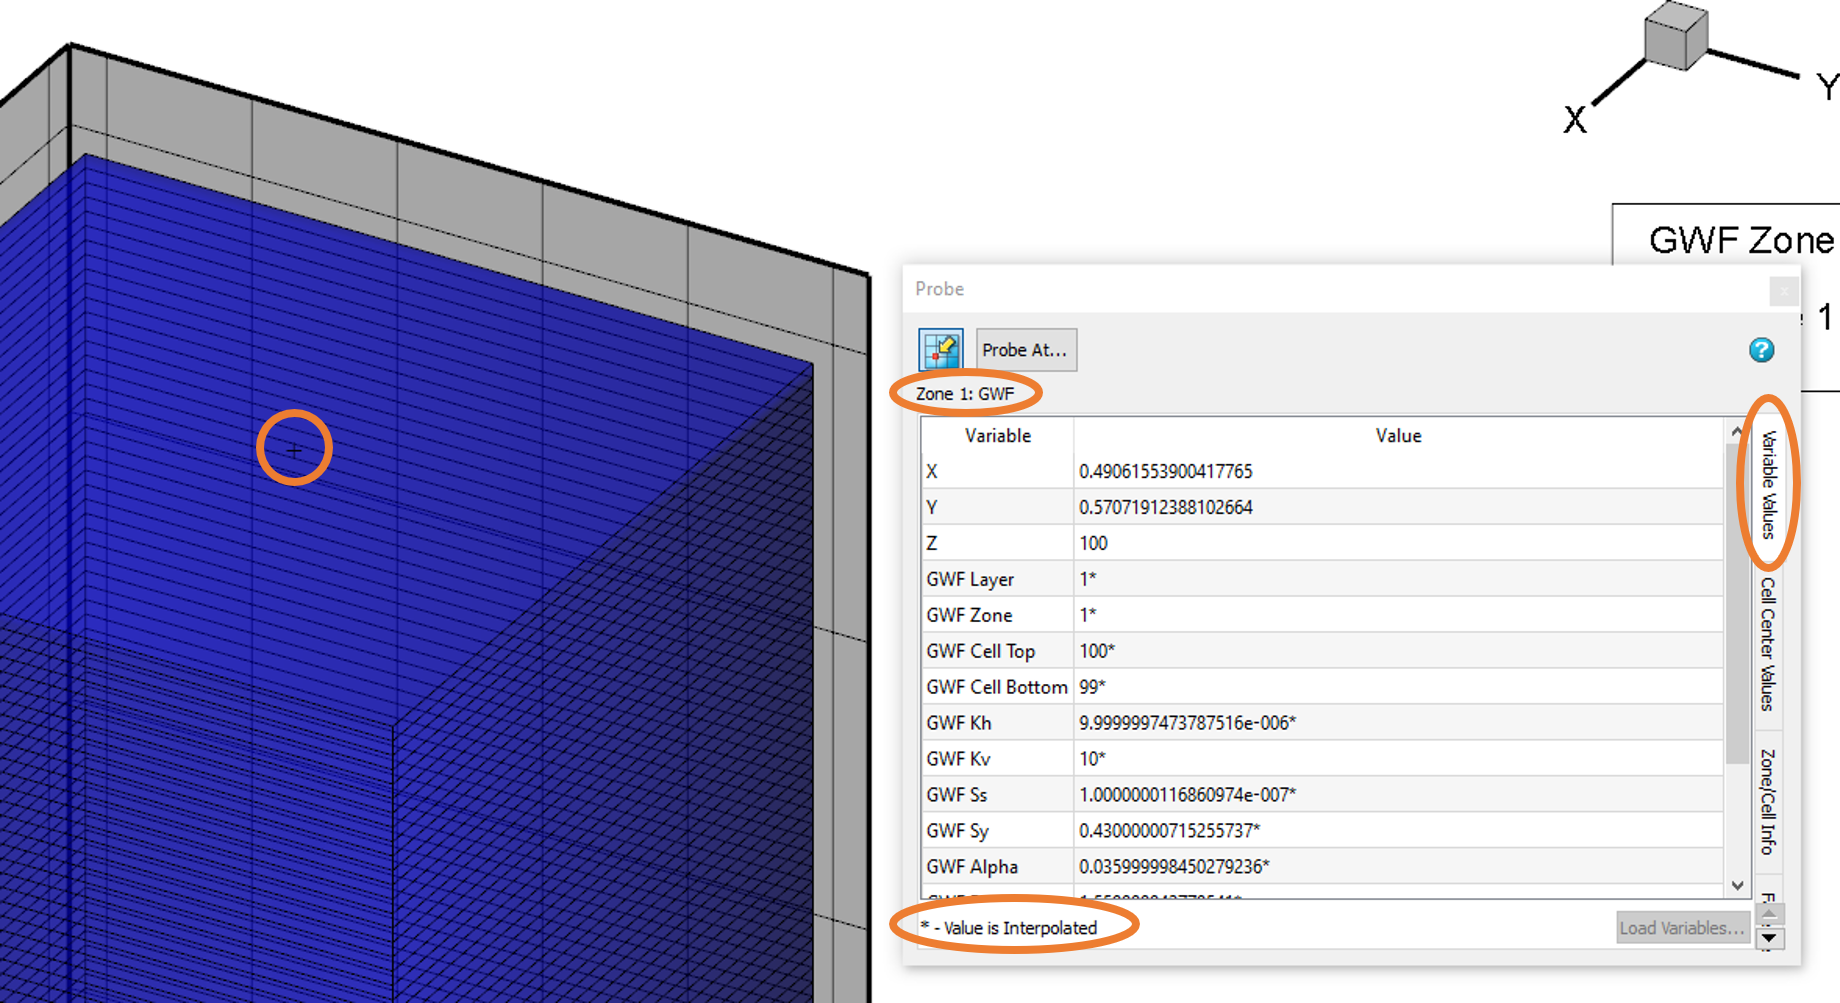
\includegraphics[width=.9\textwidth]{3_20_ProbeTool}

The probe location is indicated by the small '+' sign in the top cell (left orange circle).  This opens the {\sf Probe} dialogue which shows the zone probed ({\sf Zone 1: GWF}), and a table of  Variable names and values.

It is important to understand that in \tecplot\ nomenclature, the {\sf Variable Values} tab refers to values assigned to {\sf TMPLT\_GWF} mesh nodes, while the {\sf Cell Centred Values} tab ({\em Not to be confused with \mf\ cells!}) refers to values assigned to {\sf TMPLT\_GWF} mesh elements.

If the mesh-centred control volume approach is used, as is the case for this example, then \mf\ cell locations align with {\sf TMPLT\_GWF} mesh element centroids, and all values except the $XYZ$ coordinates (which are defined at {\sf TMPLT\_GWF} mesh nodes)  are interpolated (as indicated by an asterisk {\sf *} appended to the value}).  The $XYZ$ coordinates show the exact location of the small '+' sign.

If we select the {\sf Cell Centred Values} tab, the {\sf Probe} output looks like this:

        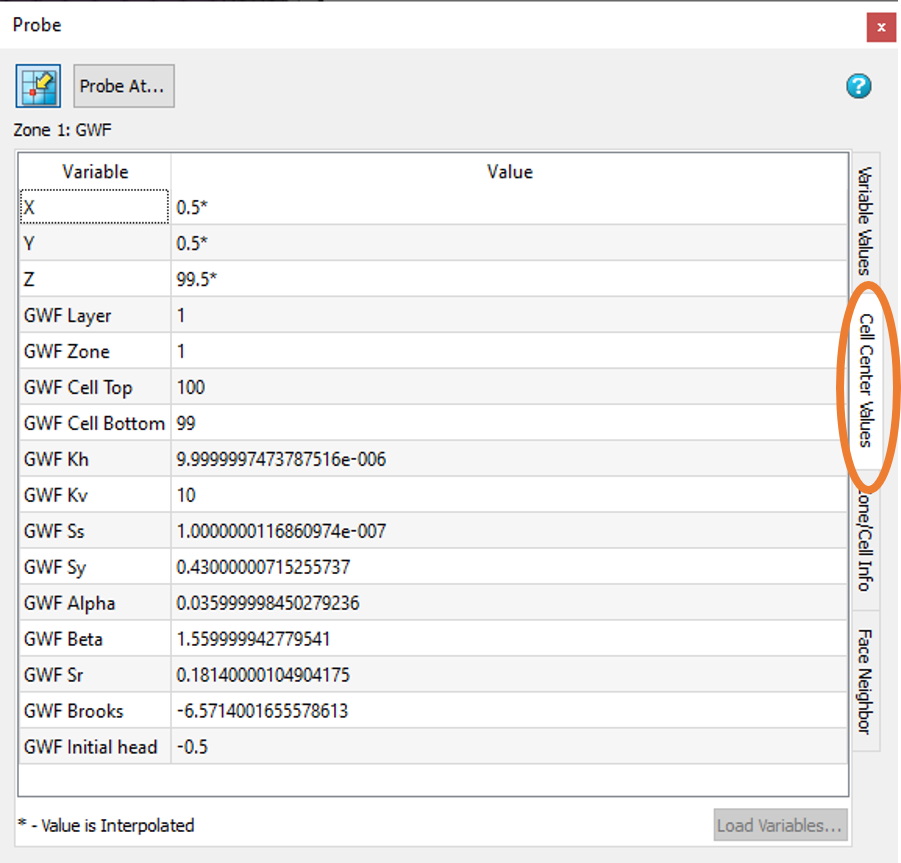
\includegraphics[width=.5\textwidth]{3_20_ProbeToolCellCentred}

Now the $XYZ$ coordinates are interpolated and show the approximate {\sf TMPLT\_GWF} mesh element centroid location, while for all other variables, exact values (i.e.\ what was input) are shown.

If the node-centred control volume approach is used, as is the case for the \texttt{6\_Abdul\_Prism\_Cell\_nc} example, then \mf\ cell locations align with {\sf TMPLT\_GWF} mesh nodes, and no variable values are interpolated when the {\sf Cell Centred Values} tab is selected.

        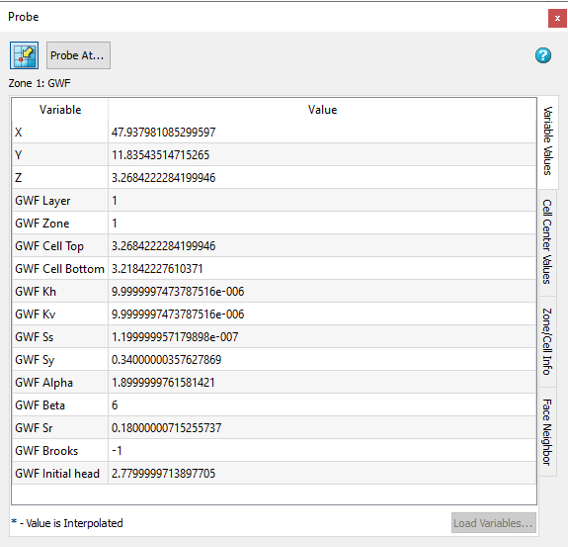
\includegraphics[width=.5\textwidth]{3_21_ProbeToolAbdul_nc}

Bring the {\sf GWF Cells} frame to the front, and send the {\sf GWF} frame to the back.

        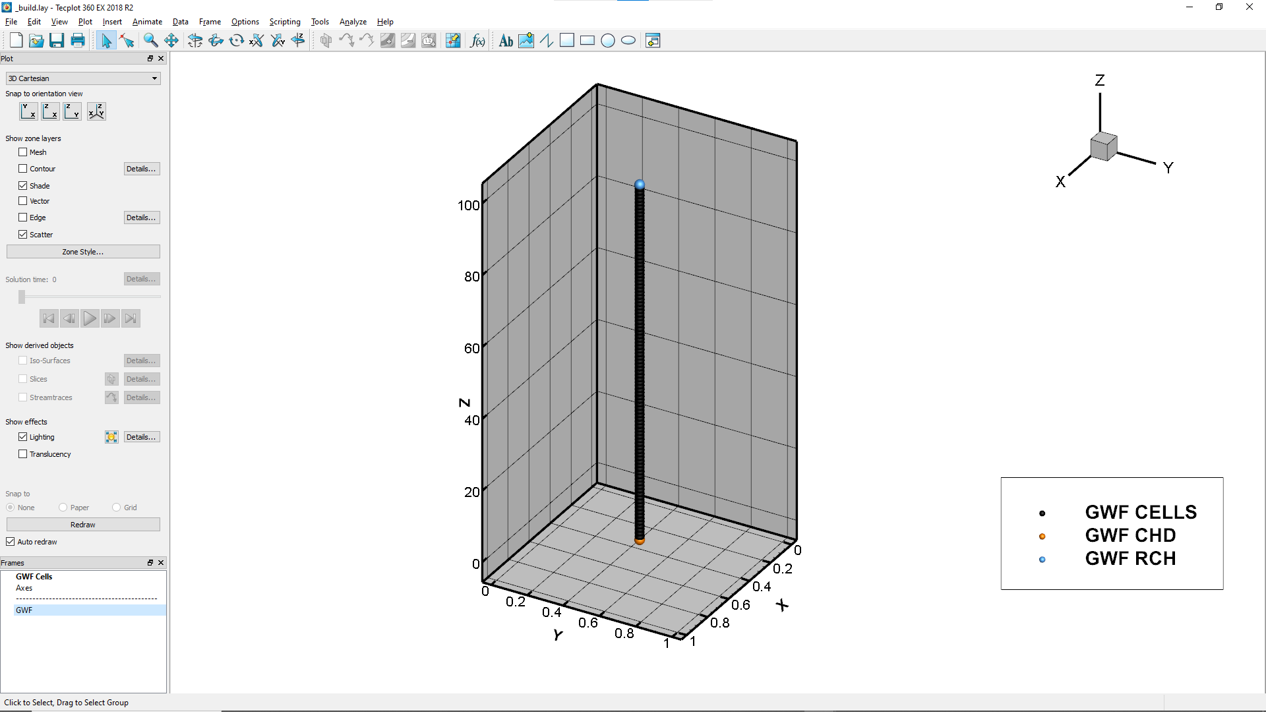
\includegraphics[width=\textwidth]{3_22_GWF_Cells}


\index{\gwf\ Domain ! {\tt \_build.lay} ! {\sf GWF Cells} frame}
The {\sf GWF Cells} frame has the following contents:
\begin{itemize}
  \item The legend, which shows three types of scatter points called {\sf GWF Cells, GWF CHD} and {\sf GWF RCH}, is shown at the middle right side.
   \item The \mfus\ cell locations are shown by the black spheres.
   \item The cell assigned recharge is shown by the large blue sphere.
   \item The cell assigned a constant head is shown by the large green sphere.
\end{itemize}

If boundary conditions are assigned to the \gwf\ domain, as they are in this case, then Tecplot output files will be produced for each type.  The {\tt \_build.lay} file has been configured to load these files.

       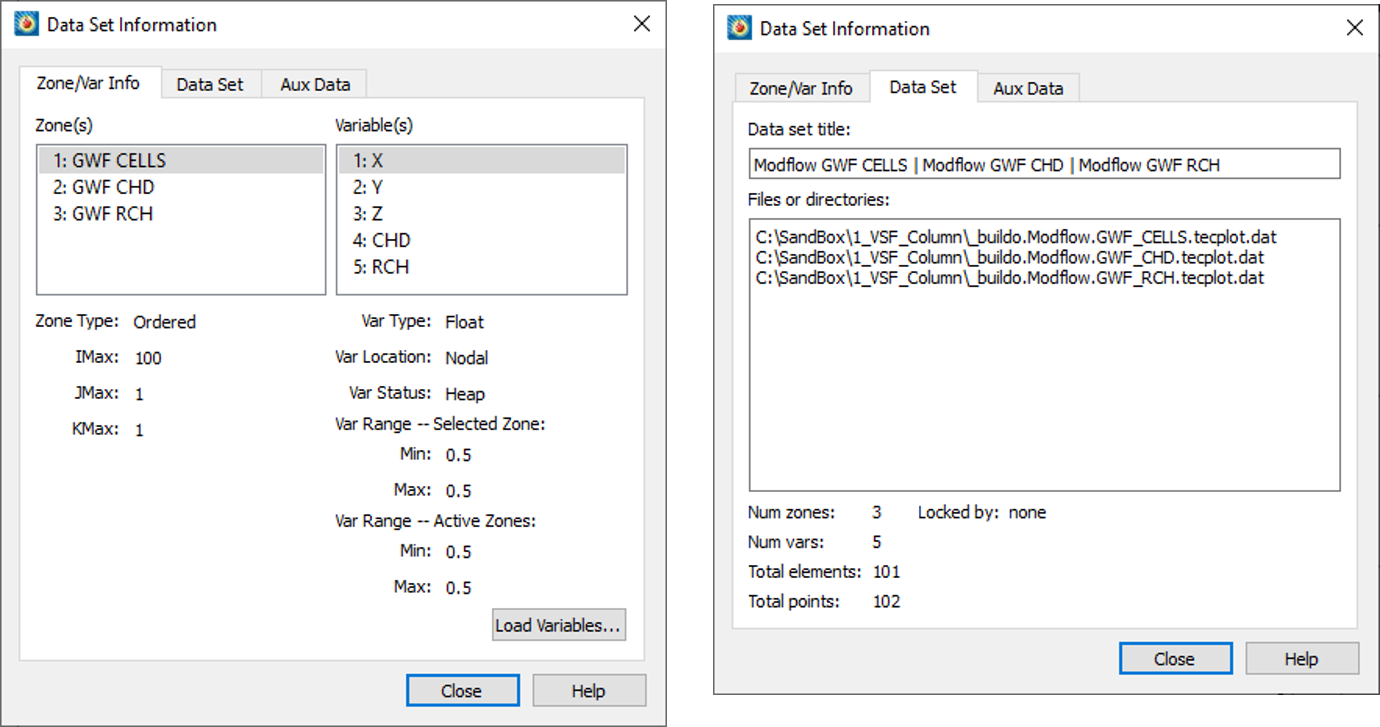
\includegraphics[width=.75\textwidth]{3_23_GWF_CellsDataInfo}

In the {\sf Zone/Var Info} tab, there are 3 zones, and 5 variables.  In the {\sf data Set} tab, we can see that 3 files have been loaded.  

Try to probe the blue sphere, and you will likely get the following warning:

       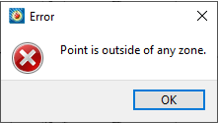
\includegraphics[width=.25\textwidth]{3_24_GWF_CellsPointOutside}

This is because the cell is located at an exact $XYZ$ point, and the chance of clicking the mouse right there is very small.  In this case, to obtain {\it exact} values for the data point nearest the specified location, hold down the {\sf Control} key while clicking the mouse at the desired location.

       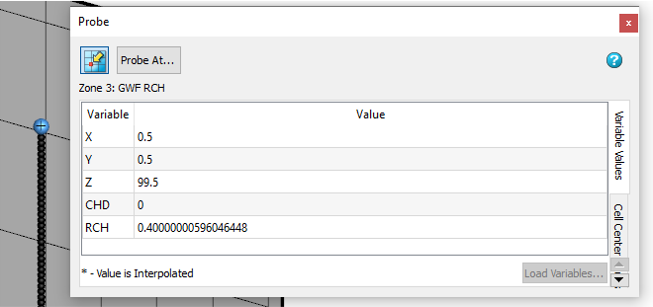
\includegraphics[width=.5\textwidth]{3_25_GWF_CellsControlClick}

You must make sure to have the {\sf Variable Values} tab selected to see values. Here, we see the $XYZ$ location of the nearest cell, and the recharge ({\sf RCH}) value 0.4.  Note that the {\sf CHD} value of 0 is shown by default at non-constant head nodes, and does not mean a constant head of zero has been assigned.   If we probe the probe the green sphere we see this. 

       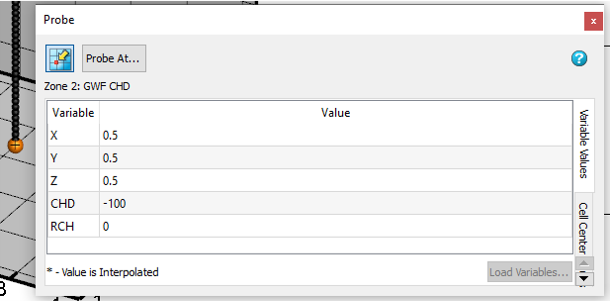
\includegraphics[width=.5\textwidth]{3_25b_GWF_CellsControlClick}

Now the constant head ({\sf CHD}) value -100 is shown while the {\sf RCH}) value is 0, because this is not an assigned recharge cell.

Since this verification example is using mesh-centred control volumes, the cells are located at the center of the finite element prisms.

The verification example \texttt{6\_Abdul\_Prism\_Cell} has a \swf\ domain defined by an irregular 2D surface with a recharge boundary condition assigned to the entire domain and a critical depth outflow boundary condition assigned at the downstream outlet. Since it also has a \gwf\ domain the {\sf \_build.lay} file is a bit more complicated, but has many of the previous example. 

Start a new command prompt, run \tecplot\ and load the {\sf \_build.lay} file.

        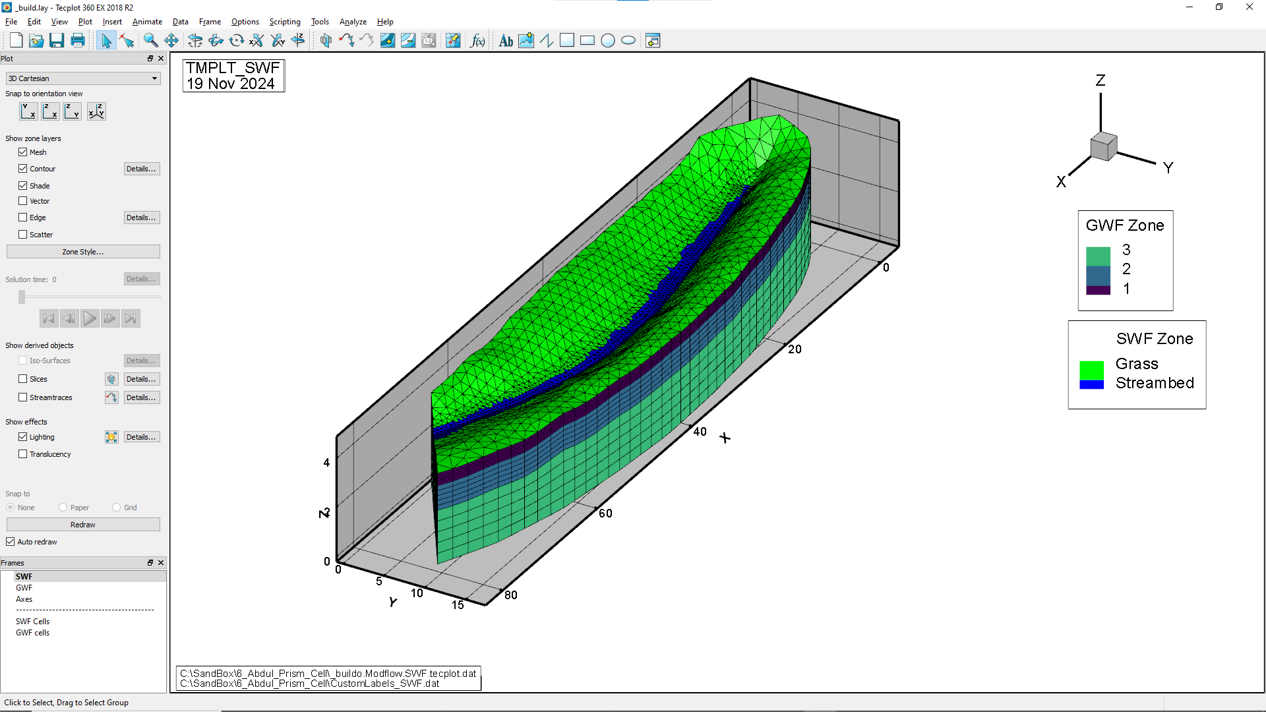
\includegraphics[width=\textwidth]{3_26_SWF_GWF}
        
Here we can see the {\sf SWF, GWF} and {\sf Axes} frames are visible (i.e. placed above the {\sf background} frame in the list).  The {\sf SWF} is currently active (i.e. the name is bolded) and placed at the front of the image (i.e. at the top of the list). It uses a different colormap to make it easier to distinguish the \gwf\ domain below.  

Send the {\sf GWF} and {\sf Axes} frames to the back to see only the contents of the {\sf SWF} frame.

        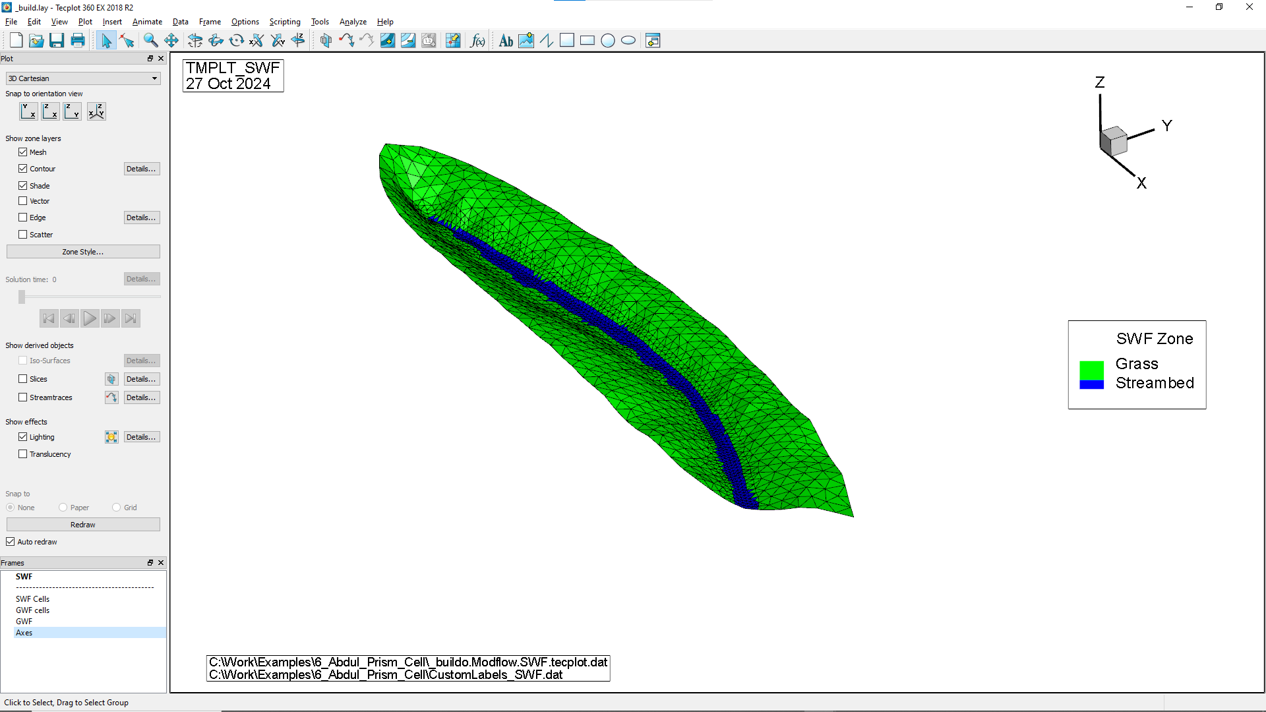
\includegraphics[width=\textwidth]{3_27_SWF}
        


\index{\swf\ Domain ! {\tt \_build.lay} ! {\sf SWF} frame}
The {\sf SWF} frame has very similar contents to the {\sf GWF} frame described earlier, but note that:
\begin{itemize}
  \item The names of the data files loaded into the frame are for the \swf\ domain.
  \item   The data set title {\sf TMPLT\_SWF} indicates that this is the \swf\ domain mesh that was created from the template mesh.
  \item The contouring legend, showing there are two \swf\ zones called {\sf Grass} and {\sf Streambed} is a bit more descriptive than e.g. {\sf Zone 1}.   These are referred to a custom labels in \tecplot.
\end{itemize}

\index{\tecplot\ ! custom labels} To define custom labels as shown for the \swf\ legend, and earlier for the \gwf\ legend, you must define a tecplot file that contains the custom label set.  This is in fact the second file loaded in the \swf\ frame called {\tt CustomLabels_SWF.dat}.  It looks like this:
\begin{verbatim}
    CUSTOMLABELS
    "Streambed",
    "Grass",
    "Zone 3",
    "Zone 4",
    "Zone 5",
    "Zone 6",
\end{verbatim}

        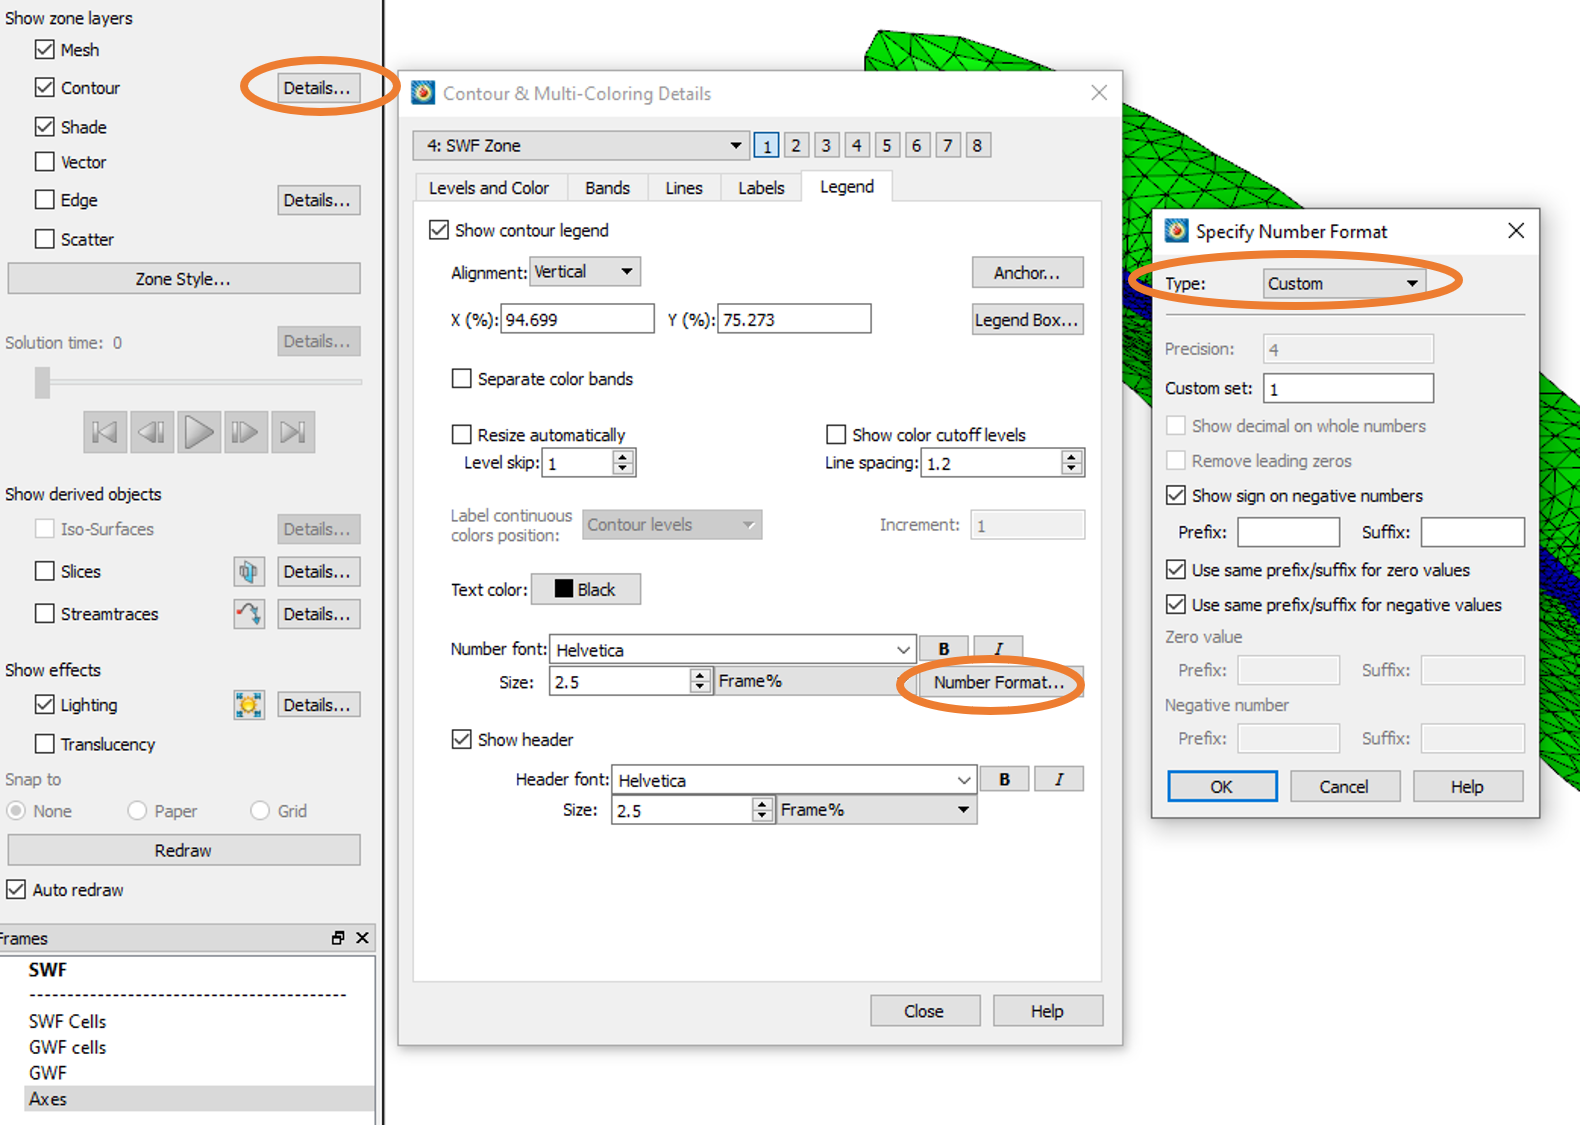
\includegraphics[width=\textwidth]{3_28_SWFCustomLabels}
        
The use of custom labels is configured by first choosing the contouring {\sf Details...} button, which opens the {\sf Contour & Multi-Coloring Details} dialogue.  Choose the {\sf Number Format...} button to open the {\sf Specify Number Format} dialogue, then choose {\sf Custom} from the {\sf Type:} drop-down menu. 


\chapter{\mfus\ Execution and Post-Processing}\label{chapter:ModelExecution}
The steps in our model excution  workflow are:
\begin{enumerate}
    \item Run \mfus to create the new project output files (e.g.\ time-varying hydraulic head, drawdown etc).\label{step:modflow}
    \item Run \mut\ to post-process the Modflow project, which produces \tecplot\ output files for the various Modflow domains (i.e.\ \gwf, \swf\ and/or \cln ) created during the Modflow simulation.\label{step:mut2}
    \item Run \tecplot\ and examine the Modflow output files.   \label{step:Tecplot2}
\end{enumerate}

To run \mfus\ on the \texttt{1\_VSF\_Column} example, and assuming we have a command prompt open at the appropriate directory, we can type:
\begin{verbatim}
    usgs_1 modflow
\end{verbatim}
which obtains the prefix for the \mfus\ input files, in this case the default prefix {\sf modflow}.

 As \mfus\ processes the input file, output is written to the screen:

        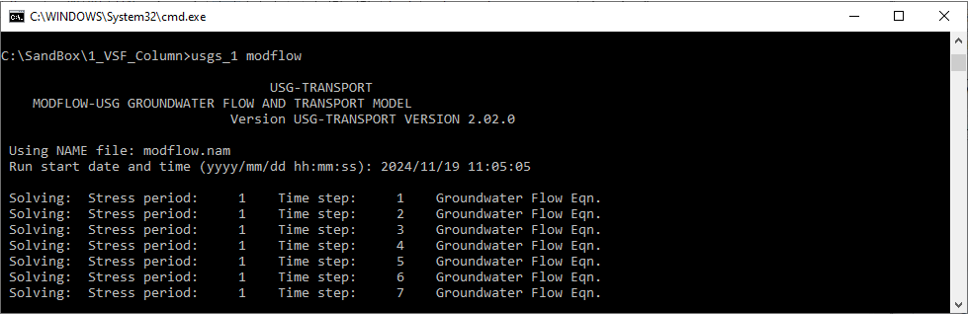
\includegraphics[width=\textwidth]{4_1_RunScreen}

 If execution is successful you will see the {\sf Normal termination of simulation} message:

        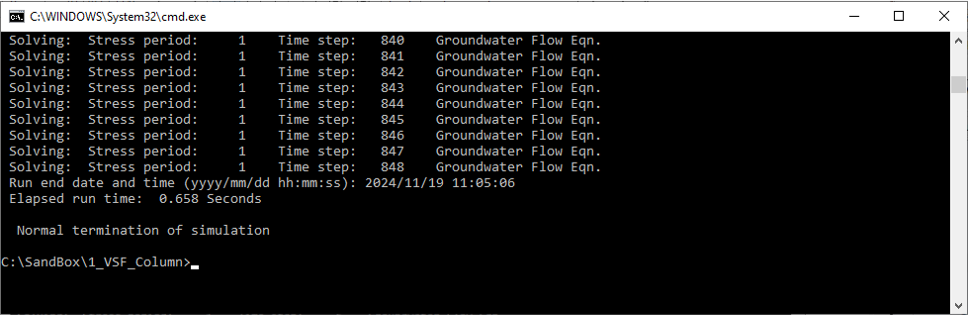
\includegraphics[width=\textwidth]{4_1_RunScreenExit}

 Every \mfus\ simulation generates a run-time
listing file, in this case called {\tt modflow.lst}, that consists of the input data for the simulation;
the solver and nonlinear outputs at user-requested detail; head
and drawdown solutions, if requested; mass-balance information; and time-step information for the simulation.  It also produces binary files of head, drawdown, saturation and cell-by-cell flows for each model domain.

To post-process the output produced by \mfus\ for the \texttt{1\_VSF\_Column} example, we would  run \mut\ using the input file \texttt{\_post.mut} by typing:
\begin{verbatim}
    mut _post
\end{verbatim}

If you open the file \texttt{\_post.mut} in a text editor you will see the first  line is a comment followed by one instruction and input:
\squish
\begin{verbatim}
    ! This example reads a modflow project and postprocesses it
    postprocess existing modflow model
        modflow
\end{verbatim}
As in the model build, \mut\ first creates a clean copy of the input file called \texttt{\_posto.input} by removing all comment lines.
 As it processes the input file, output is written to both the screen and to the file \texttt{\_posto.eco}.

The instruction to post-process the \mfus\ model after execution is:

\ins{postprocess existing modflow model}
    {
        \squish
        \begin{enumerate}
        \item \str{Prefix}  The \mfus\ model prefix.
        \end{enumerate}
        Given \str{Prefix}, this instruction:
         \begin{itemize}
            \item  Reads head, drawdown and cell-by-cell flow binary output files for each output time and writes the results to the file {\tt \_posto.modflow.GWF.tecplot.dat}
            \item scans the \mfus\ listing file, extracts volumetric budget data at each time step and writes the results to the file {\tt \_posto.modflow.VolumeBudget.tecplot.dat}
         \end{itemize}
        \squish
    }

\index{Volumetric water budget}
Volumetric water budget data is useful for checking the fluid mass balance of the model run.  The example {\tt 4\_SWF\_RCH\_CRD} has a \tecplot\ layout file {\tt VolumetricBudget.lay} which you can load directly into \tecplot\ from the command prompt by typing:
    \begin{verbatim}
        tec360 VolumetricBudget.lay
    \end{verbatim}

        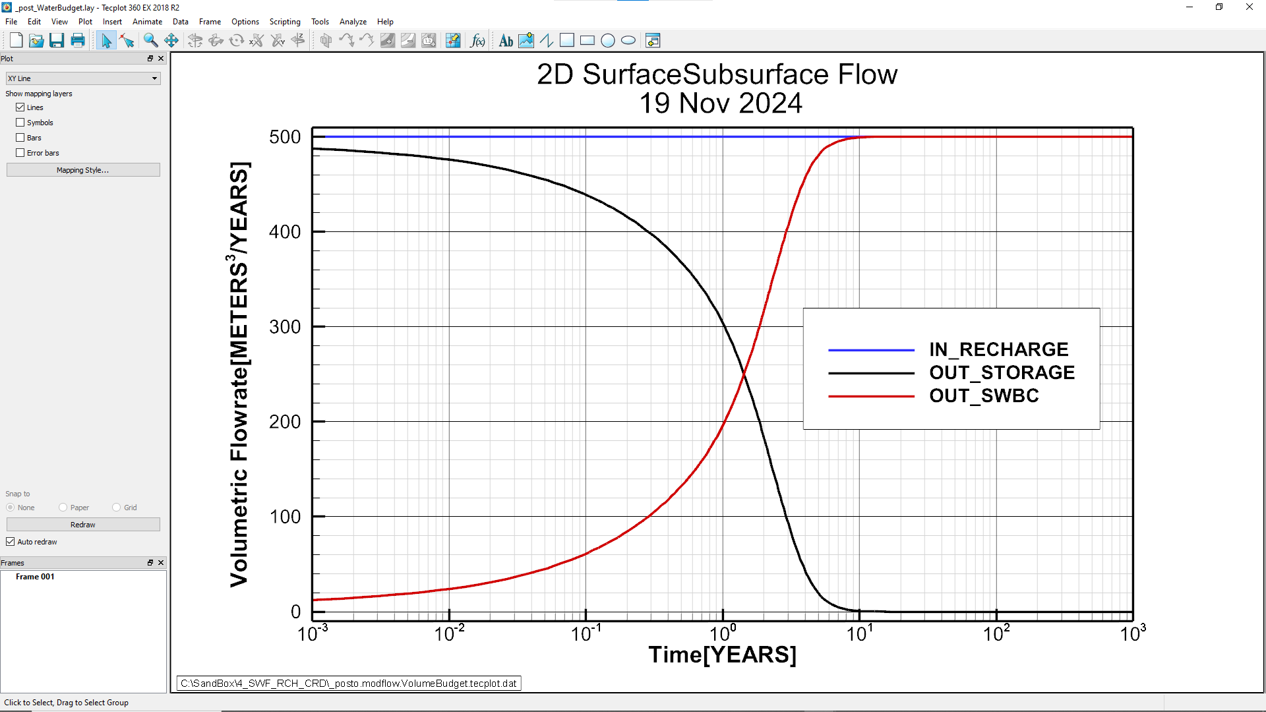
\includegraphics[width=\textwidth]{4_2_Budget}

This \tecplot\ frame has the following features and contents:
\begin{itemize}
  \item It is an {\sf XY Line} plot showing the volumetric flowrate versus time for selected components of the model.
  \item The name of the data file loaded into the frame is shown at the bottom left corner.
  \item The plot title, current date (on the day the file was loaded) and data set title ({\sf 4\_SWF\_RCH\_CRD}) are shown centred above the plot.
  \item The line legend is shown on the right side of the plot.
  \item The X-axis uses a log time scale.
\end{itemize}

The \tecplot\ date set information dialogue shows all of the variables available for plotting:

        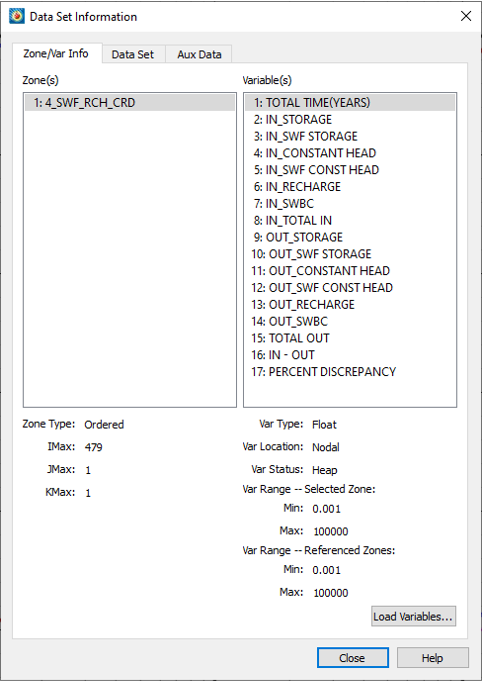
\includegraphics[width=.6\textwidth]{4_3_DataSetInfo}

Variable names are derived from the {\tt modflow.lst} file:
\begin{verbatim}
      VOLUMETRIC BUDGET FOR ENTIRE MODEL AT END OF TIME STEP  479 IN STRESS PERIOD    1
      ----------------------------------------------------------------------------- ---

         CUMULATIVE VOLUMES      L**3       RATES FOR THIS TIME STEP      L**3/T
         ------------------                 ------------------------

               IN:                                      IN:
               ---                                      ---
                 STORAGE =       3.0881E-04               STORAGE =       5.6023E-09
             SWF STORAGE =       9.9743E-03           SWF STORAGE =       2.1841E-13
           CONSTANT HEAD =           0.0000         CONSTANT HEAD =           0.0000
          SWF CONST HEAD =           0.0000        SWF CONST HEAD =           0.0000
                RECHARGE =    50000000.0000              RECHARGE =         500.0000
                    SWBC =           0.0000                  SWBC =           0.0000

                TOTAL IN =    50000000.0103              TOTAL IN =         500.0000

        ... etc

     PERCENT DISCREPANCY =           0.01     PERCENT DISCREPANCY =           0.01
\end{verbatim}


This example has a uniform recharge rate of 0.5 $meters/year$ which results in a total recharge of 500 $meters^{3}/year$ when multiplied by the 1000 $meter$ length of the cross-section. Initially, water comes out of storage then but this declines to zero at equilibrium.  Water exiting the surface water outflow critical depth boundary  {\sf OUT\_SWBC} is initially zero then rises to equal the toal recharge at equilibrium.  Fluid balance error {\sf IN-OUT} is essentially zero throughout the simulation.

The probe tool can be used in {\sf XY Line} plots to get exact variable values at a chosen location along the X or Y axis.  The cursor is shown as a vertical line if probing values on the X-axis (i.e.\ over time):

        \includegraphics[width=\textwidth]{4_4_Probe}

Here, the location of the probe is shown by small vertical lines placed where the probe crossed the plotted lines.  The exact coordinate is given as {\sf X1: 0.2967...}  years.  At this early time, the {\sf OUT\_STORAGE} value is still near its initial value of 500 and the {\sf OUT\_SWBC} has just started rising.

A \tecplot\ layout file, \texttt{\_post.lay}, has been created for each verification example and  provides a quick way to view \mfus\ model solution results.  This result is from the example {\tt 6\_Abdul\_Prism\_Cell}:

        \includegraphics[width=\textwidth]{4_5_Post_Abdul}

The {\tt \_post.lay} layout file is similar to the {\tt \_build.lay} file shown earlier for the same problem: {\sf  SWF, GWF} and {\sf Axes} frames are visible (i.e. placed above the {\sf background} frame in the list).  The {\sf SWF} is currently active (i.e. the name is bolded) and placed at the front of the image (i.e. at the top of the list). It uses a different colormap to make it easier to distinguish the \gwf\ domain below.

In this case though, the contoured variables are {\sf SWF Depth} and {\sf GWF Saturation} results from the \mfus\ simulation.  The model output includes data for several output times, and the image above is showing conditions at a solution time of 3000 seconds, as indicated by the label near the top center of the plot.  The solution time shown is controlled by the slider and button controls near the centre of the {\sf Plot} frame on the left hand side of the image:

        \includegraphics[width=.8\textwidth]{4_6_SolutionSlider}

The {\sf Details...} button leads to the {\sf Time animation details} dialogue which allows you to control and save animations of transient model results using the {\sf Export To File} button \includegraphics{ExportToFile}.  There is an example animation in  \texttt{$\backslash$MUT\_Examples-main$\backslash$\-6\_Abdul\_Prism\_Cell} folder in the powerpoint file {\tt Abdul Problem Animation.pptx}.  It used the settings shown in the {\sf Export} dialogue above to limit animations speed and write to an {\tt AVI}-formatted file.  This was then inserted in powerpoint where it can be viewed.

The {\sf Data Set Information} dialogues for the {\sf SWF} and {\sf GWF} frames are shown below:

        \includegraphics[width=.8\textwidth]{4_7_DatSetInfo}

These are similar to those shown earlier during the model build except there are now multiple {\sf Zone(s)}, one for each output time.  The {\sf Solution Time} (6000) is shown for the highlighted zone, in this case zone 10.

Included are these cell properties:
\begin{itemize}
    \item Elevation {\sf SWF z Cell} and {\sf GWF z Cell}.
    \item \mf\ layer number  {\sf SWF layer}and {\sf GWF layer}.
    \item \mf\ boundary number {\sf SWF Ibound} and {\sf GWF Ibound}.
    \item Initial head.
    \item Hydraulic head result.
    \item \gwf\ saturation and \swf\ depth.  These are stored in the \mf\ DDN (drawdown) file.
    \item In this case, cell-by-cell flows are stored in \gwf\ variables 10 to 13 and \swf\ variables 10 to 15.
\end{itemize}

The verification example {\tt 6\_Abdul\_MODHMS} layout file {\sf \_plot.lay} uses \tecplot\ value-blanking and the {\sf SWF Ibound} and {\sf GWF Ibound} to remove inactive cells, which have an IBOUND value of 0, from the plot:

        \includegraphics[width=.8\textwidth]{4_7a_MODHMS}


        \includegraphics[width=.8\textwidth]{4_7b_ValueBlanking}

\index{\tecplot\ ! value blanking} 


        \includegraphics[width=.8\textwidth]{4_8_Slices}

\index{\tecplot\ ! slices and Fence diagrams}



\chapter{Model Verification}\label{chapter:ModelVerification} 
    \section{1D Variably-saturated Flow in a Column} \label{section:1d_column_example}
This example \footnote{See verification example   \texttt{MUT\_Examples$\backslash$1\_VSF\_Column}} simulates variably-saturated flow in a 1D column of homogeneous sand 100 m thick.
Parameter values used in this example are shown in Table~\ref{tab:column}.
    \begin{table}
        \centering
        \caption{Parameter Values for Simulation of the 1-D Column.}
        \begin{tabular}{lll}  \hline
            Parameter                             & Value & Unit                           \\ \hline
            specific yield (porosity)             &  0.34                    &             \\
            hydraulic conductivity                &  $ 1 \times 10^{-5}$     &m s$^{-1}$  \\
            specific storage coefficient          &  $ 1.2 \times 10^{-7}$   & m$^{-1}$   \\
            Van Genuchten parameter               &  1.9                     &m$^{-1}$     \\
            Van Genuchten parameter               &  6                       &             \\
            residual saturation                   &  0.18                    &             \\
%            Brooks-Corey coefficient              &  3.4                     &             \\
            Manning coefficient for plot          &  0.3                     &s m$^{-1/3}$ \\
            Manning coefficient for channel       &  0.03                    &s m$^{-1/3}$ \\
            Initial water table elevation         &  2.78                    &m            \\
        \hline
        \end{tabular}
        \label{tab:column}
    \end{table}

The Van Genuchten unsaturated function type was used.

A uniform rainfall of 0.4 m/s was applied to the top of the column and the base was fixed at a pressure head of -100 m.

    \pagebreak
    Here is a comparison of pressure head versus depth results for  \mfus\ and \hgs\ at 20 and 40 seconds:
    \vspace{.2in} \\
    \includegraphics[width=0.87\textwidth]{1d_P_vs_Z}
    \vspace{.2in} \\

    Here is a comparison of saturation versus depth results for  \mfus\ and \hgs\ at 20 and 40 seconds:
    \vspace{.2in} \\
    \includegraphics[width=0.87\textwidth]{1d_S_vs_Z}
    \vspace{.2in} \\

%\includegraphics[width=.15\textwidth]{UnderConstruction} \textit{
%Although these results look good, there is a discrepancy between the unit systems used in the two models (e.g. K is 10 in \hgs\ and 1e-5 in \mfus.   HGS column height appears to be 100 cm, while \mfus\ model is 100 m thick.
%\mut\ needs to be modified to allow the user to change unit systems and then we should update this example.
%}





    \section{2D Variably-saturated Flow in a Hillslope: Drains vs Surfacewater Flow} \input{2D_Hillslope}
    \section{3D Fully-coupled Groundwater-Surface Water Flow: Abdul's Experiment}\label{section:3D_Example_Abdul}
These three examples simulate the fully three-dimensional surface/subsurface flows observed in  experiments conducted at Canadian Forces Base Borden, in Ontario, Canada, by Abdul (1985):
\begin{description}
    \item [Example 1 (\texttt{6\_Abdul\_Prism\_Cell)}:] A fully-coupled \gwf-\swf\ system receives recharge to the \swf\ domain and allows drainage from \swf\ cells located at the downstream outflow boundary.
        The template and \swf\ meshes are composed of 3-node triangular elements while the \gwf\ mesh is composed of 6-node prismatic elements.  The mesh-centred control volume approach is used to define the \mfus\ cells.
    \item [Example 2 (\texttt{\_Abdul\_Prism\_Cell\_nc}):] Similar to example 2 except the node-centred control volume approach is used to define the \mfus\ cells.
    \item [Example 3 (\texttt{6\_Abdul\_MODHMS}):] Similar to example 1 except The template and \swf\ meshes are composed of 4-node rectangular elements while the \gwf\ mesh is composed of 8-node hexahedral elements.
\end{description}

The following parameter values were used for the \gwf\ domain in all 3 examples:

\begin{center}
    \begin{tabular}{lll}  \hline
        Parameter                             & Value                       &     Unit                                \\ \hline
        Specific yield (porosity)             &  0.34                       &                   \\
        Hydraulic conductivity                &  $ 1 \times 10^{-5}$        &     m s$^{-1}$    \\
        Specific storage coefficient          &  $ 1.2 \times 10^{-7}$      &     m$^{-1}$      \\
        Van Genuchten Alpha                   &  1.9                        &     m$^{-1}$      \\
        Van Genuchten Beta                    &  6                          &                   \\
        Residual saturation                   &  0.18                     &                   \\
    \hline
    \end{tabular}
\end{center}

The Van Genuchten unsaturated function type was used.

For examples 1 and 2, the \swf\ domain was subdivided into 2 zones called grass and streambed as shown here for example 1:

\includegraphics[width=0.7\textwidth]{5_7_SWFZones}

These parameter values were used for the grass zone for example 1 and 2:

\begin{center}
    \begin{tabular}{lll}  \hline
        Parameter                           & Value                         &   Unit            \\ \hline
        Manning's coefficient               &  0.3                          &   s m$^{-1/3}$   \\
        Depression storage height           &  0.1                          &   m               \\
        Obstruction storage height          &  0.0                          &   m               \\
        Depth for smoothing height 1        &  $1 \times 10^{-6}$     &   m               \\
        Depth for smoothing height 2        &  $1 \times 10^{-6}$     &   m               \\
    \hline
    \end{tabular}
\end{center}

These parameter values were calibrated and used for the streambed zone in examples 1 an 2:

\begin{center}
    \begin{tabular}{lll}  \hline
        Parameter                           & Value                         &   Unit            \\ \hline
        Manning's coefficient               &  0.01                         &   s m$^{-1/3}$   \\
        Depression storage height           &  0.1                          &   m               \\
        Obstruction storage height          &  0.0                          &   m               \\
        Depth for smoothing height 1        &  $3.75334 \times 10^{-3}$     &   m               \\
        Depth for smoothing height 2        &  $1.26394 \times 10^{-3}$     &   m               \\
    \hline
    \end{tabular}
\end{center}

Example 3 used a single \swf\ zone, which used these calibrated parameter values:

\begin{center}
    \begin{tabular}{lll}  \hline
        Parameter                           & Value                         &   Unit            \\ \hline
        Manning's coefficient               &  0.02                         &   s m$^{-1/3}$   \\
        Depression storage height           &  0.1                          &   m               \\
        Obstruction storage height          &  0.0                          &   m               \\
        Depth for smoothing height 1        &  $1.19106 \times 10^{-2}$     &   m               \\
        Depth for smoothing height 2        &  $2.49907 \times 10^{-2}$     &   m               \\
    \hline
    \end{tabular}
\end{center}

The 3 examples shared the following initial and boundary conditions:
\begin{itemize}
    \item An initial head of 2.78 m was assigned to the \gwf\ domain.
    \item An initial surface water depth of $1 \times 10^{-3}$  m was assigned to the \swf\ domain.
    \item A recharge of $5.56 \times 10^{-6}$ m/s was applied to the \swf\ domain for a time of 3000 s (stress period 1) then the recharge was reduced to 0.0 m/s for an additional 3000 s (stress period 2).
    \item A critical depth boundary was assigned to selected \swf\ cells located at the downstream end of the stream channel.
\end{itemize}

\pagebreak
Here is a comparison of measured and simulated stream outflow versus time for the Abdul field study.

\includegraphics[width=0.87\textwidth]{5_8_Abdul_Outflow_3_Examples}

Simulation results are presented for the 3 examples as well as from \hgs\ and {\sc Modflow-Surfact}.  The results are similar for all cases.




%\chapter{Illustrative Example} \label{chapter:IllustrativeExample}
%\includegraphics[width=.15\textwidth]{UnderConstruction} \textit{
%We intend to present a watershed scale example of a fully-coupled \gwf\-\swf\ system.
%}


\appendix

\chapter{\excel\ Database Files}\label{Appendix:ExcelUseage}
\excel\ files are used to store information in the following databases:
\begin{itemize}
  \item \texttt{GWF.xlsx} for \gwf\ domain material parameters.
  \item \texttt{SWF.xlsx} for \swf\ domain material parameters.
  \item \texttt{CLN.xlsx} for \cln\ domain material parameters.
  \item \texttt{SMS.xlsx} for solver parameters.
  \item \texttt{ET.xlsx} and  \texttt{LAI.xlsx} for evapotranspiration (ET) and leaf area index (LAI) parameters respectively.  {\em These are currently just placeholders for future development and will not be discussed further at this time.}
\end{itemize}

Modifications can be made to the database by editing the \texttt{xlsx} file in \excel\ and exporting the results to a \texttt{csv}-formatted version of the file which is then read and processed by \mut.  We will use the \gwf\ database to illustrate the modification workflow, which can then be applied to the other databases.

If you are a \mut\ end-user, you should edit the database files in the \bin\ directory, as outlined on page~\pageref{page:userbin}.

If you are a developer and have downloaded the MUT\_Examples repository, you should edit the database files in the directory \textit{pathto}\texttt{$\backslash$Grdbldr$\backslash$\_MUT\_USERBIN},
where the string \textit{pathto} represents the local path to the repository (e.g.\ \texttt{c:$\backslash$repos}).

First, open the \texttt{GWF.xlsx} in \excel:

    \includegraphics[width=\textwidth]{Excel_1_GWFxlsx}

Some key features to note are:
\begin{itemize}
    \item The first row contains database field (i.e.\ column) names.
    \item The existing database contains data for 10 materials stored in rows 2 to 11.
\end{itemize}

As a precaution, the database is protected. \index{Excel ! cell protection} If you try to modify any of the existing contents, in this case rows 1 to 11, you will receive the following warning:

    \includegraphics[width=\textwidth]{Excel_2_ProtectionWarning}

To unprotect the sheet, choose {\sf Review}, then {\sf Unprotect sheet}:

   \includegraphics[width=.7\textwidth]{Excel_3_unprotect}

You will be prompted to enter a password, which is {\tt mut}.

To protect the sheet, choose {\sf Review}, then {\sf Protect sheet}, then enter and confirm a password.  We suggest you use the {\tt mut} password.  If not, don't forget the new password!

The purpose for protecting the database is to prevent accidental changes from being made to critical material properties so future runs referring to protected material ID's yield repeatable results.  This would be the case, for example,  for material properties calibrated for an engineering project or verification example, which occupy the first 6 materials in this \gwf\ database).

Although the database is protected, you can add your own materials starting at row 12.  The easiest way to add a material is to copy an existing one.  For example, we can copy row 10 (silt) to row 12:
\begin{enumerate}
    \item Click on the number {\sf 10} at the left end of row 10 to select the entire row.

   \includegraphics[width=\textwidth]{Excel_4_select}

    \item Type {\tt ctrl-C} to copy it.
    \item Click on the number {\sf 12} at the left end of row 12 to select the entire row.
    \item Type {\tt ctrl-V} to paste it.

   \includegraphics[width=\textwidth]{Excel_5_Paste}

\end{enumerate}
Note that the new material ID number is automatically set to 11, which is the previous number of materials plus 1. You should now change the material name and properties as desired.

If you want to extend the zone of protected cells to include the added row 12 you should do the following:
\begin{enumerate}
    \item Unprotect the worksheet.
    \item Select the entire worksheet by pressing {\tt ctrl-A} or clicking on the \includegraphics{Excel_SelectAll} button at the top left corner of the worksheet.
    \item {\tt Right-click} on any cell and choose {\sf Format cells...} from the drop-down menu, then in the {\sf Protection} tab uncheck the {\sf Locked} checkbox then choose {\sf OK}.

        \includegraphics[width=.7\textwidth]{Excel_5b_FormatCells}
    \item Select only the cells containing data that you want to protect, in this case from columns {\sf A} to {\sf P} and rows {\sf 1} to {\sf 12}.
    \item {\tt Right-click} on any chosen cell, choose {\sf Format cells...} from the drop-down menu, then  in the {\sf Protection} tab check the {\sf Locked} checkbox then choose {\sf OK}.
    \item Protect the worksheet.
\end{enumerate}

Columns {\sf I, N} and {\sf O} are special fields where the input is restricted by a list of choices.  For example, if you click on cell {\sf I12}, the {\sf Unsaturated Function Type} for the new material, you will see a drop-down list button \includegraphics{Excel_DropListArrow} appear beside the cell.  To choose, for example, the {\sf van Genuchten} function type, select the button and highlight the option in the list and press enter:

   \includegraphics[width=.2\textwidth]{Excel_6_list}

The second worksheet, {\sf Options}, contains the following data:

   \includegraphics[width=.6\textwidth]{Excel_7_Options}

These are the drop-down lists for the unsaturated function type, length unit, time unit in fields I, N and O respectively.  This worksheet is also protected with the password {\tt mut}.

Once you have finished modifying the material properties, you should save the \texttt{xlsx} file, then export them to a \texttt{csv} file by:
\begin{enumerate}
    \item Selecting {\sf File/Export/Change File Type/CSV}:

   \includegraphics[width=\textwidth]{Excel_8_export}

   \item  Selecting {\sf CSV (Comma delimited)(*.csv)}
   \item  {\tt Clicking} the {\sf Save As} button.
\end{enumerate}






%\chapter{\tecplot\ Useage}\label{tecfile:TecplotUseage} 
%\chapter{\github\ Useage in \vstudio} \label{tutorial:GitInVStudio}


\printindex
\newpage

%\input{CookingNotes}
%\input{Scans}



\end{document}

% -----------------------------------------------------------------------------
